\documentclass[twoside]{book}

% Packages required by doxygen
\usepackage{fixltx2e}
\usepackage{calc}
\usepackage{doxygen}
\usepackage[export]{adjustbox} % also loads graphicx
\usepackage{graphicx}
\usepackage[utf8]{inputenc}
\usepackage{makeidx}
\usepackage{multicol}
\usepackage{multirow}
\PassOptionsToPackage{warn}{textcomp}
\usepackage{textcomp}
\usepackage[nointegrals]{wasysym}
\usepackage[table]{xcolor}

% Font selection
\usepackage[T1]{fontenc}
\usepackage[scaled=.90]{helvet}
\usepackage{courier}
\usepackage{amssymb}
\usepackage{sectsty}
\renewcommand{\familydefault}{\sfdefault}
\allsectionsfont{%
  \fontseries{bc}\selectfont%
  \color{darkgray}%
}
\renewcommand{\DoxyLabelFont}{%
  \fontseries{bc}\selectfont%
  \color{darkgray}%
}
\newcommand{\+}{\discretionary{\mbox{\scriptsize$\hookleftarrow$}}{}{}}

% Page & text layout
\usepackage{geometry}
\geometry{%
  a4paper,%
  top=2.5cm,%
  bottom=2.5cm,%
  left=2.5cm,%
  right=2.5cm%
}
\tolerance=750
\hfuzz=15pt
\hbadness=750
\setlength{\emergencystretch}{15pt}
\setlength{\parindent}{0cm}
\setlength{\parskip}{3ex plus 2ex minus 2ex}
\makeatletter
\renewcommand{\paragraph}{%
  \@startsection{paragraph}{4}{0ex}{-1.0ex}{1.0ex}{%
    \normalfont\normalsize\bfseries\SS@parafont%
  }%
}
\renewcommand{\subparagraph}{%
  \@startsection{subparagraph}{5}{0ex}{-1.0ex}{1.0ex}{%
    \normalfont\normalsize\bfseries\SS@subparafont%
  }%
}
\makeatother

% Headers & footers
\usepackage{fancyhdr}
\pagestyle{fancyplain}
\fancyhead[LE]{\fancyplain{}{\bfseries\thepage}}
\fancyhead[CE]{\fancyplain{}{}}
\fancyhead[RE]{\fancyplain{}{\bfseries\leftmark}}
\fancyhead[LO]{\fancyplain{}{\bfseries\rightmark}}
\fancyhead[CO]{\fancyplain{}{}}
\fancyhead[RO]{\fancyplain{}{\bfseries\thepage}}
\fancyfoot[LE]{\fancyplain{}{}}
\fancyfoot[CE]{\fancyplain{}{}}
\fancyfoot[RE]{\fancyplain{}{\bfseries\scriptsize Generated by Doxygen }}
\fancyfoot[LO]{\fancyplain{}{\bfseries\scriptsize Generated by Doxygen }}
\fancyfoot[CO]{\fancyplain{}{}}
\fancyfoot[RO]{\fancyplain{}{}}
\renewcommand{\footrulewidth}{0.4pt}
\renewcommand{\chaptermark}[1]{%
  \markboth{#1}{}%
}
\renewcommand{\sectionmark}[1]{%
  \markright{\thesection\ #1}%
}

% Indices & bibliography
\usepackage{natbib}
\usepackage[titles]{tocloft}
\setcounter{tocdepth}{3}
\setcounter{secnumdepth}{5}
\makeindex

% Hyperlinks (required, but should be loaded last)
\usepackage{ifpdf}
\ifpdf
  \usepackage[pdftex,pagebackref=true]{hyperref}
\else
  \usepackage[ps2pdf,pagebackref=true]{hyperref}
\fi
\hypersetup{%
  colorlinks=true,%
  linkcolor=blue,%
  citecolor=blue,%
  unicode%
}

% Custom commands
\newcommand{\clearemptydoublepage}{%
  \newpage{\pagestyle{empty}\cleardoublepage}%
}

\usepackage{caption}
\captionsetup{labelsep=space,justification=centering,font={bf},singlelinecheck=off,skip=4pt,position=top}

%===== C O N T E N T S =====

\begin{document}

% Titlepage & ToC
\hypersetup{pageanchor=false,
             bookmarksnumbered=true,
             pdfencoding=unicode
            }
\pagenumbering{alph}
\begin{titlepage}
\vspace*{7cm}
\begin{center}%
{\Large My Project }\\
\vspace*{1cm}
{\large Generated by Doxygen 1.8.13}\\
\end{center}
\end{titlepage}
\clearemptydoublepage
\pagenumbering{roman}
\tableofcontents
\clearemptydoublepage
\pagenumbering{arabic}
\hypersetup{pageanchor=true}

%--- Begin generated contents ---
\chapter{Rent-\/\+A-\/\+Ride}
\label{md__r_e_a_d_m_e}
\Hypertarget{md__r_e_a_d_m_e}
3112 Final Project 
\chapter{Hierarchical Index}
\section{Class Hierarchy}
This inheritance list is sorted roughly, but not completely, alphabetically\+:\begin{DoxyCompactList}
\item \contentsline{section}{Customer}{\pageref{class_customer}}{}
\item \contentsline{section}{Rental\+Manager}{\pageref{class_rental_manager}}{}
\item \contentsline{section}{Vehicle}{\pageref{class_vehicle}}{}
\begin{DoxyCompactList}
\item \contentsline{section}{Car}{\pageref{class_car}}{}
\item \contentsline{section}{Motorcycle}{\pageref{class_motorcycle}}{}
\item \contentsline{section}{S\+UV}{\pageref{class_s_u_v}}{}
\item \contentsline{section}{Truck}{\pageref{class_truck}}{}
\end{DoxyCompactList}
\end{DoxyCompactList}

\chapter{Class Index}
\section{Class List}
Here are the classes, structs, unions and interfaces with brief descriptions\+:\begin{DoxyCompactList}
\item\contentsline{section}{\hyperlink{class_car}{Car} }{\pageref{class_car}}{}
\item\contentsline{section}{\hyperlink{class_customer}{Customer} }{\pageref{class_customer}}{}
\item\contentsline{section}{\hyperlink{class_motorcycle}{Motorcycle} }{\pageref{class_motorcycle}}{}
\item\contentsline{section}{\hyperlink{class_rental_manager}{Rental\+Manager} }{\pageref{class_rental_manager}}{}
\item\contentsline{section}{\hyperlink{class_s_u_v}{S\+UV} }{\pageref{class_s_u_v}}{}
\item\contentsline{section}{\hyperlink{class_truck}{Truck} }{\pageref{class_truck}}{}
\item\contentsline{section}{\hyperlink{class_vehicle}{Vehicle} }{\pageref{class_vehicle}}{}
\end{DoxyCompactList}

\chapter{File Index}
\section{File List}
Here is a list of all documented files with brief descriptions\+:\begin{DoxyCompactList}
\item\contentsline{section}{\hyperlink{car_8cpp}{car.\+cpp} \\*I\+T\+CS 3112 Rent-\/\+A-\/\+Ride Final Project }{\pageref{car_8cpp}}{}
\item\contentsline{section}{\hyperlink{car_8h}{car.\+h} \\*I\+T\+CS 3112 Rent-\/\+A-\/\+Ride Final Project }{\pageref{car_8h}}{}
\item\contentsline{section}{\hyperlink{customer_8h}{customer.\+h} \\*I\+T\+CS 3112 Final Project }{\pageref{customer_8h}}{}
\item\contentsline{section}{\hyperlink{motorcycle_8cpp}{motorcycle.\+cpp} \\*I\+T\+CS 3112 Rent-\/\+A-\/\+Ride Final Project }{\pageref{motorcycle_8cpp}}{}
\item\contentsline{section}{\hyperlink{motorcycle_8h}{motorcycle.\+h} \\*I\+T\+CS 3112 Rent-\/\+A-\/\+Ride Final Project }{\pageref{motorcycle_8h}}{}
\item\contentsline{section}{\hyperlink{_ra_r_g_u_i_8cpp}{Ra\+R\+G\+U\+I.\+cpp} \\*I\+T\+CS 3112 Rent-\/\+A-\/\+Ride Final Project }{\pageref{_ra_r_g_u_i_8cpp}}{}
\item\contentsline{section}{\hyperlink{rental_manager_8cpp}{rental\+Manager.\+cpp} \\*I\+T\+CS 3112 Rent-\/\+A-\/\+Ride Final Project }{\pageref{rental_manager_8cpp}}{}
\item\contentsline{section}{\hyperlink{rental_manager_8h}{rental\+Manager.\+h} \\*I\+T\+CS 3112 Final Project }{\pageref{rental_manager_8h}}{}
\item\contentsline{section}{\hyperlink{suv_8cpp}{suv.\+cpp} \\*I\+T\+CS 3112 Rent-\/\+A-\/\+Ride Final Project }{\pageref{suv_8cpp}}{}
\item\contentsline{section}{\hyperlink{suv_8h}{suv.\+h} \\*I\+T\+CS 3112 Rent-\/\+A-\/\+Ride Final Project }{\pageref{suv_8h}}{}
\item\contentsline{section}{\hyperlink{truck_8cpp}{truck.\+cpp} \\*I\+T\+CS 3112 Rent-\/\+A-\/\+Ride Final Project }{\pageref{truck_8cpp}}{}
\item\contentsline{section}{\hyperlink{truck_8h}{truck.\+h} \\*I\+T\+CS 3112 Rent-\/\+A-\/\+Ride Final Project }{\pageref{truck_8h}}{}
\item\contentsline{section}{\hyperlink{vehicle_8cpp}{vehicle.\+cpp} \\*I\+T\+CS 3112 Rent-\/\+A-\/\+Ride Final Project }{\pageref{vehicle_8cpp}}{}
\item\contentsline{section}{\hyperlink{vehicle_8h}{vehicle.\+h} \\*I\+T\+CS 3112 Rent-\/\+A-\/\+Ride Final Project }{\pageref{vehicle_8h}}{}
\end{DoxyCompactList}

\chapter{Class Documentation}
\hypertarget{class_car}{}\section{Car Class Reference}
\label{class_car}\index{Car@{Car}}
Inheritance diagram for Car\+:\begin{figure}[H]
\begin{center}
\leavevmode
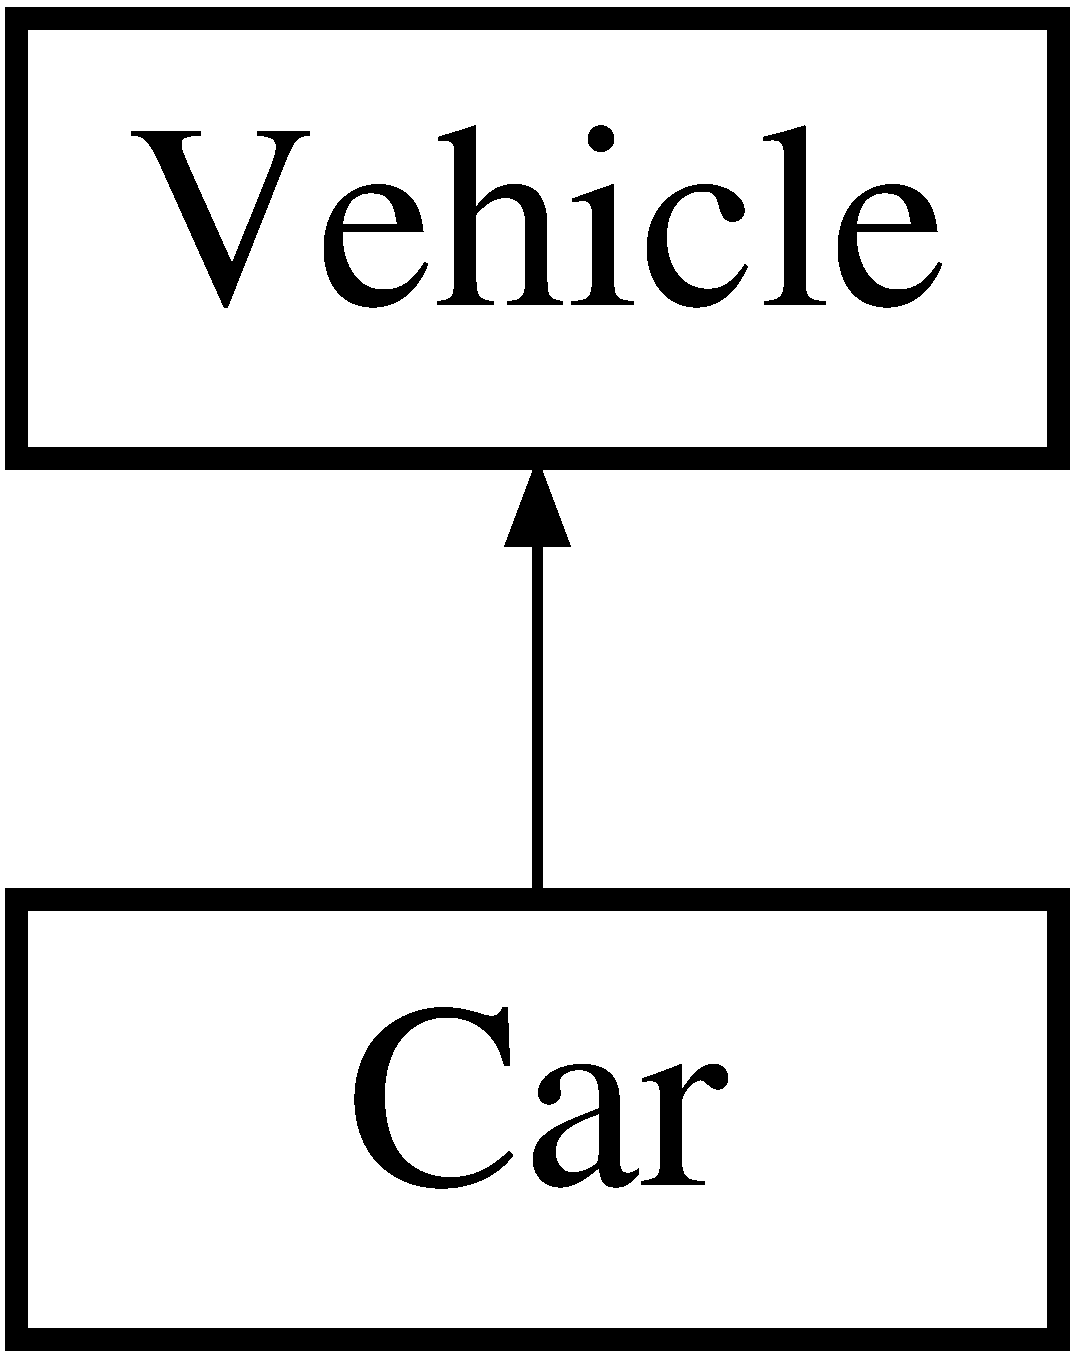
\includegraphics[height=2.000000cm]{class_car}
\end{center}
\end{figure}
\subsection*{Public Member Functions}
\begin{DoxyCompactItemize}
\item 
\hyperlink{class_car_a1c803f7c5038d3e31b368b0d0a35493c}{Car} ()
\item 
\hyperlink{class_car_a618f4d3c9a4edd09cb6477db71266fdd}{Car} (string make, string model, int year, string color, int num\+Wheels, int customer\+ID, int status, string type)
\item 
\hyperlink{class_car_a5933bb06e96b159fe339a128abda888a}{$\sim$\+Car} ()
\end{DoxyCompactItemize}
\subsection*{Additional Inherited Members}


\subsection{Constructor \& Destructor Documentation}
\mbox{\Hypertarget{class_car_a1c803f7c5038d3e31b368b0d0a35493c}\label{class_car_a1c803f7c5038d3e31b368b0d0a35493c}} 
\index{Car@{Car}!Car@{Car}}
\index{Car@{Car}!Car@{Car}}
\subsubsection{\texorpdfstring{Car()}{Car()}\hspace{0.1cm}{\footnotesize\ttfamily [1/2]}}
{\footnotesize\ttfamily Car\+::\+Car (\begin{DoxyParamCaption}{ }\end{DoxyParamCaption})}

\hyperlink{class_car}{Car} class constructor. \mbox{\Hypertarget{class_car_a618f4d3c9a4edd09cb6477db71266fdd}\label{class_car_a618f4d3c9a4edd09cb6477db71266fdd}} 
\index{Car@{Car}!Car@{Car}}
\index{Car@{Car}!Car@{Car}}
\subsubsection{\texorpdfstring{Car()}{Car()}\hspace{0.1cm}{\footnotesize\ttfamily [2/2]}}
{\footnotesize\ttfamily Car\+::\+Car (\begin{DoxyParamCaption}\item[{string}]{make,  }\item[{string}]{model,  }\item[{int}]{year,  }\item[{string}]{color,  }\item[{int}]{num\+Wheels,  }\item[{int}]{customer\+ID,  }\item[{int}]{status,  }\item[{string}]{type }\end{DoxyParamCaption})}

\hyperlink{class_car}{Car} class constructor takes in several parameters that apply to a \hyperlink{class_car}{Car} object. \mbox{\Hypertarget{class_car_a5933bb06e96b159fe339a128abda888a}\label{class_car_a5933bb06e96b159fe339a128abda888a}} 
\index{Car@{Car}!````~Car@{$\sim$\+Car}}
\index{````~Car@{$\sim$\+Car}!Car@{Car}}
\subsubsection{\texorpdfstring{$\sim$\+Car()}{~Car()}}
{\footnotesize\ttfamily Car\+::$\sim$\+Car (\begin{DoxyParamCaption}{ }\end{DoxyParamCaption})}

Destructor 

The documentation for this class was generated from the following files\+:\begin{DoxyCompactItemize}
\item 
\hyperlink{car_8h}{car.\+h}\item 
\hyperlink{car_8cpp}{car.\+cpp}\end{DoxyCompactItemize}

\hypertarget{class_customer}{}\section{Customer Class Reference}
\label{class_customer}\index{Customer@{Customer}}
\subsection*{Public Member Functions}
\begin{DoxyCompactItemize}
\item 
\hyperlink{class_customer_abcc8fae9701e5ba9d7d6fe44498b34e3}{Customer} ()
\item 
\hyperlink{class_customer_a0e0e31707d01bf721067c7a73b5bea8c}{Customer} (string first\+Name, string last\+Name, int custoer\+ID)
\item 
void \hyperlink{class_customer_aad7bbf65329d9ad4bc4a99cb5ed8fdbd}{set\+First\+Name} (string first\+Name)
\item 
string \hyperlink{class_customer_a406993fb9cf665aa2b44355de7c12d58}{get\+First\+Name} ()
\item 
void \hyperlink{class_customer_a16bda3871286ed4ff13400dbd988790a}{set\+Last\+Name} (string last\+Name)
\item 
string \hyperlink{class_customer_aef91fec461e6d0ad72ef3162b8711b76}{get\+Last\+Name} ()
\item 
void \hyperlink{class_customer_af17373c7df70e19949f35274bef0071e}{set\+Customer\+ID} (int customer\+ID)
\item 
int \hyperlink{class_customer_a236d5d040cafabeb6f84296d3e101ff1}{get\+Customer\+ID} ()
\item 
string \hyperlink{class_customer_a09a36773263493f72efc4b3f02648c03}{to\+String} ()
\end{DoxyCompactItemize}


\subsection{Constructor \& Destructor Documentation}
\mbox{\Hypertarget{class_customer_abcc8fae9701e5ba9d7d6fe44498b34e3}\label{class_customer_abcc8fae9701e5ba9d7d6fe44498b34e3}} 
\index{Customer@{Customer}!Customer@{Customer}}
\index{Customer@{Customer}!Customer@{Customer}}
\subsubsection{\texorpdfstring{Customer()}{Customer()}\hspace{0.1cm}{\footnotesize\ttfamily [1/2]}}
{\footnotesize\ttfamily Customer\+::\+Customer (\begin{DoxyParamCaption}{ }\end{DoxyParamCaption})}

\hyperlink{class_customer}{Customer} class constructor. \mbox{\Hypertarget{class_customer_a0e0e31707d01bf721067c7a73b5bea8c}\label{class_customer_a0e0e31707d01bf721067c7a73b5bea8c}} 
\index{Customer@{Customer}!Customer@{Customer}}
\index{Customer@{Customer}!Customer@{Customer}}
\subsubsection{\texorpdfstring{Customer()}{Customer()}\hspace{0.1cm}{\footnotesize\ttfamily [2/2]}}
{\footnotesize\ttfamily Customer\+::\+Customer (\begin{DoxyParamCaption}\item[{string}]{first\+Name,  }\item[{string}]{last\+Name,  }\item[{int}]{customer\+ID }\end{DoxyParamCaption})}

\hyperlink{class_customer}{Customer} class constructor takes in strings first\+Name and last\+Name and int customer\+ID to populate those parameters for a specific customer. 

\subsection{Member Function Documentation}
\mbox{\Hypertarget{class_customer_a236d5d040cafabeb6f84296d3e101ff1}\label{class_customer_a236d5d040cafabeb6f84296d3e101ff1}} 
\index{Customer@{Customer}!get\+Customer\+ID@{get\+Customer\+ID}}
\index{get\+Customer\+ID@{get\+Customer\+ID}!Customer@{Customer}}
\subsubsection{\texorpdfstring{get\+Customer\+I\+D()}{getCustomerID()}}
{\footnotesize\ttfamily int Customer\+::get\+Customer\+ID (\begin{DoxyParamCaption}{ }\end{DoxyParamCaption})}

Fucntion returns the customer\+ID of \hyperlink{class_customer}{Customer}. \begin{DoxyReturn}{Returns}
customer\+ID 
\end{DoxyReturn}
\mbox{\Hypertarget{class_customer_a406993fb9cf665aa2b44355de7c12d58}\label{class_customer_a406993fb9cf665aa2b44355de7c12d58}} 
\index{Customer@{Customer}!get\+First\+Name@{get\+First\+Name}}
\index{get\+First\+Name@{get\+First\+Name}!Customer@{Customer}}
\subsubsection{\texorpdfstring{get\+First\+Name()}{getFirstName()}}
{\footnotesize\ttfamily string Customer\+::get\+First\+Name (\begin{DoxyParamCaption}{ }\end{DoxyParamCaption})}

Fucntion returns the first\+Name of \hyperlink{class_customer}{Customer}. \begin{DoxyReturn}{Returns}
first\+Name 
\end{DoxyReturn}
\mbox{\Hypertarget{class_customer_aef91fec461e6d0ad72ef3162b8711b76}\label{class_customer_aef91fec461e6d0ad72ef3162b8711b76}} 
\index{Customer@{Customer}!get\+Last\+Name@{get\+Last\+Name}}
\index{get\+Last\+Name@{get\+Last\+Name}!Customer@{Customer}}
\subsubsection{\texorpdfstring{get\+Last\+Name()}{getLastName()}}
{\footnotesize\ttfamily string Customer\+::get\+Last\+Name (\begin{DoxyParamCaption}{ }\end{DoxyParamCaption})}

Fucntion returns the last\+Name of \hyperlink{class_customer}{Customer}. \begin{DoxyReturn}{Returns}
last\+Name 
\end{DoxyReturn}
\mbox{\Hypertarget{class_customer_af17373c7df70e19949f35274bef0071e}\label{class_customer_af17373c7df70e19949f35274bef0071e}} 
\index{Customer@{Customer}!set\+Customer\+ID@{set\+Customer\+ID}}
\index{set\+Customer\+ID@{set\+Customer\+ID}!Customer@{Customer}}
\subsubsection{\texorpdfstring{set\+Customer\+I\+D()}{setCustomerID()}}
{\footnotesize\ttfamily void Customer\+::set\+Customer\+ID (\begin{DoxyParamCaption}\item[{int}]{customer\+ID }\end{DoxyParamCaption})}

Function populates customer\+ID with integer. 
\begin{DoxyParams}{Parameters}
{\em customer\+ID} & \\
\hline
\end{DoxyParams}
\begin{DoxyReturn}{Returns}
none 
\end{DoxyReturn}
\mbox{\Hypertarget{class_customer_aad7bbf65329d9ad4bc4a99cb5ed8fdbd}\label{class_customer_aad7bbf65329d9ad4bc4a99cb5ed8fdbd}} 
\index{Customer@{Customer}!set\+First\+Name@{set\+First\+Name}}
\index{set\+First\+Name@{set\+First\+Name}!Customer@{Customer}}
\subsubsection{\texorpdfstring{set\+First\+Name()}{setFirstName()}}
{\footnotesize\ttfamily void Customer\+::set\+First\+Name (\begin{DoxyParamCaption}\item[{string}]{first\+Name }\end{DoxyParamCaption})}

Function populates first\+Name with string. 
\begin{DoxyParams}{Parameters}
{\em first\+Name} & \\
\hline
\end{DoxyParams}
\begin{DoxyReturn}{Returns}
none 
\end{DoxyReturn}
\mbox{\Hypertarget{class_customer_a16bda3871286ed4ff13400dbd988790a}\label{class_customer_a16bda3871286ed4ff13400dbd988790a}} 
\index{Customer@{Customer}!set\+Last\+Name@{set\+Last\+Name}}
\index{set\+Last\+Name@{set\+Last\+Name}!Customer@{Customer}}
\subsubsection{\texorpdfstring{set\+Last\+Name()}{setLastName()}}
{\footnotesize\ttfamily void Customer\+::set\+Last\+Name (\begin{DoxyParamCaption}\item[{string}]{last\+Name }\end{DoxyParamCaption})}

Function populates last\+Name with string. 
\begin{DoxyParams}{Parameters}
{\em first\+Name} & \\
\hline
\end{DoxyParams}
\begin{DoxyReturn}{Returns}
none 
\end{DoxyReturn}
\mbox{\Hypertarget{class_customer_a09a36773263493f72efc4b3f02648c03}\label{class_customer_a09a36773263493f72efc4b3f02648c03}} 
\index{Customer@{Customer}!to\+String@{to\+String}}
\index{to\+String@{to\+String}!Customer@{Customer}}
\subsubsection{\texorpdfstring{to\+String()}{toString()}}
{\footnotesize\ttfamily string Customer\+::to\+String (\begin{DoxyParamCaption}{ }\end{DoxyParamCaption})}

Fucntion returns a string formated to \char`\"{}first\+Name last\+Name customer\+I\+D\char`\"{} 

The documentation for this class was generated from the following files\+:\begin{DoxyCompactItemize}
\item 
\hyperlink{customer_8h}{customer.\+h}\item 
customer.\+cpp\end{DoxyCompactItemize}

\hypertarget{class_motorcycle}{}\section{Motorcycle Class Reference}
\label{class_motorcycle}\index{Motorcycle@{Motorcycle}}
Inheritance diagram for Motorcycle\+:\begin{figure}[H]
\begin{center}
\leavevmode
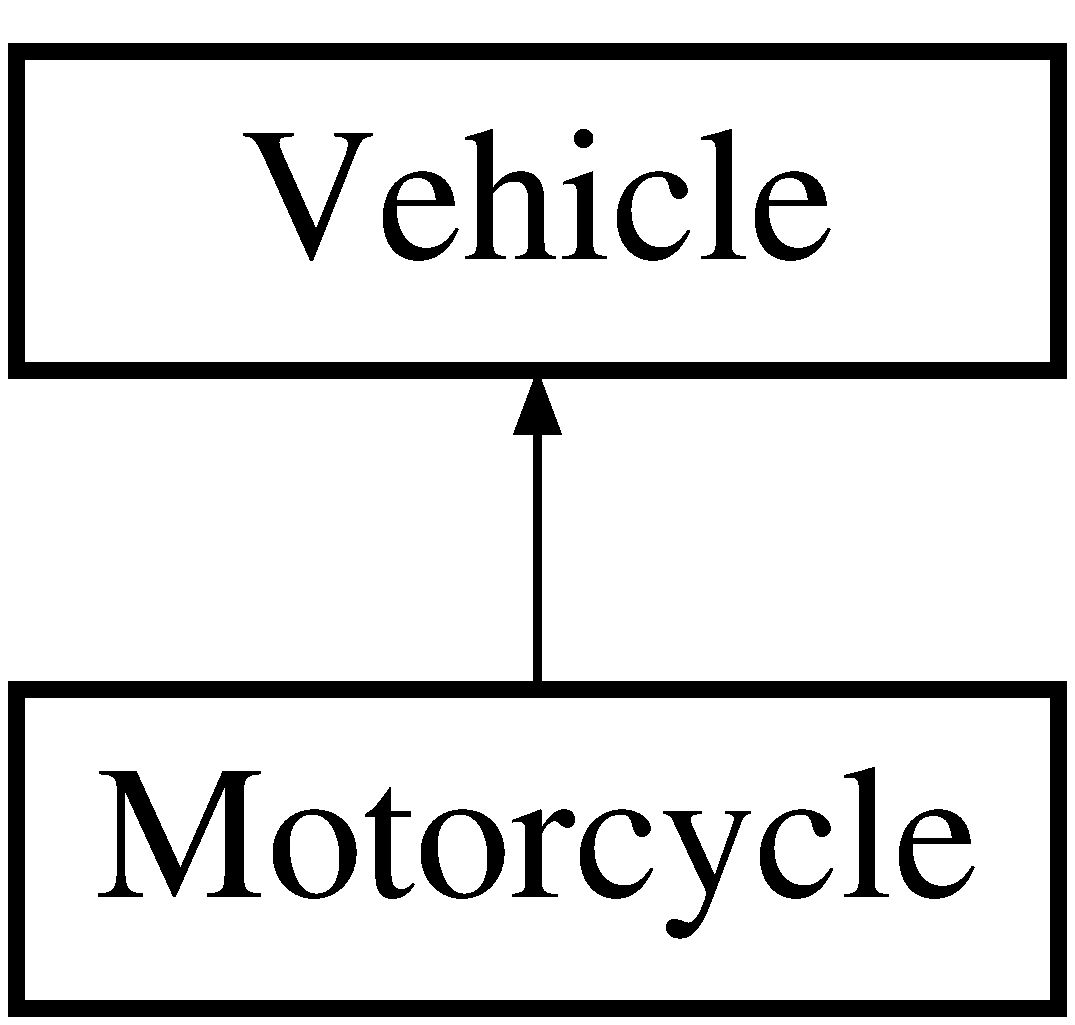
\includegraphics[height=2.000000cm]{class_motorcycle}
\end{center}
\end{figure}
\subsection*{Public Member Functions}
\begin{DoxyCompactItemize}
\item 
\hyperlink{class_motorcycle_a5682a8a6156b3337eabb3a70fd59f2d6}{Motorcycle} ()
\item 
\hyperlink{class_motorcycle_ae3f0c6f4817595fea8e0486d51d12f73}{Motorcycle} (string make, string model, int year, string color, int num\+Wheels, int customer\+Num, int status, string type)
\item 
\hyperlink{class_motorcycle_ae202420292e8ce9745243b70bf873664}{$\sim$\+Motorcycle} ()
\end{DoxyCompactItemize}
\subsection*{Additional Inherited Members}


\subsection{Constructor \& Destructor Documentation}
\mbox{\Hypertarget{class_motorcycle_a5682a8a6156b3337eabb3a70fd59f2d6}\label{class_motorcycle_a5682a8a6156b3337eabb3a70fd59f2d6}} 
\index{Motorcycle@{Motorcycle}!Motorcycle@{Motorcycle}}
\index{Motorcycle@{Motorcycle}!Motorcycle@{Motorcycle}}
\subsubsection{\texorpdfstring{Motorcycle()}{Motorcycle()}\hspace{0.1cm}{\footnotesize\ttfamily [1/2]}}
{\footnotesize\ttfamily Motorcycle\+::\+Motorcycle (\begin{DoxyParamCaption}{ }\end{DoxyParamCaption})}

\hyperlink{class_motorcycle}{Motorcycle} class constructor. \mbox{\Hypertarget{class_motorcycle_ae3f0c6f4817595fea8e0486d51d12f73}\label{class_motorcycle_ae3f0c6f4817595fea8e0486d51d12f73}} 
\index{Motorcycle@{Motorcycle}!Motorcycle@{Motorcycle}}
\index{Motorcycle@{Motorcycle}!Motorcycle@{Motorcycle}}
\subsubsection{\texorpdfstring{Motorcycle()}{Motorcycle()}\hspace{0.1cm}{\footnotesize\ttfamily [2/2]}}
{\footnotesize\ttfamily Motorcycle\+::\+Motorcycle (\begin{DoxyParamCaption}\item[{string}]{make,  }\item[{string}]{model,  }\item[{int}]{year,  }\item[{string}]{color,  }\item[{int}]{num\+Wheels,  }\item[{int}]{customer\+ID,  }\item[{int}]{status,  }\item[{string}]{type }\end{DoxyParamCaption})}

\hyperlink{class_motorcycle}{Motorcycle} class constructor takes in several parameters that apply to a \hyperlink{class_motorcycle}{Motorcycle} object. \mbox{\Hypertarget{class_motorcycle_ae202420292e8ce9745243b70bf873664}\label{class_motorcycle_ae202420292e8ce9745243b70bf873664}} 
\index{Motorcycle@{Motorcycle}!````~Motorcycle@{$\sim$\+Motorcycle}}
\index{````~Motorcycle@{$\sim$\+Motorcycle}!Motorcycle@{Motorcycle}}
\subsubsection{\texorpdfstring{$\sim$\+Motorcycle()}{~Motorcycle()}}
{\footnotesize\ttfamily Motorcycle\+::$\sim$\+Motorcycle (\begin{DoxyParamCaption}{ }\end{DoxyParamCaption})}

Destructor 

The documentation for this class was generated from the following files\+:\begin{DoxyCompactItemize}
\item 
\hyperlink{motorcycle_8h}{motorcycle.\+h}\item 
\hyperlink{motorcycle_8cpp}{motorcycle.\+cpp}\end{DoxyCompactItemize}

\hypertarget{class_rental_manager}{}\section{Rental\+Manager Class Reference}
\label{class_rental_manager}\index{Rental\+Manager@{Rental\+Manager}}
\subsection*{Public Member Functions}
\begin{DoxyCompactItemize}
\item 
\hyperlink{class_rental_manager_a2e8eabdde863514dd4ca13a5e3a4e533}{Rental\+Manager} ()
\item 
\hyperlink{class_rental_manager_a0c8562369e957400e17bd176ee18c91f}{Rental\+Manager} (string vehicles, string customers)
\item 
void \hyperlink{class_rental_manager_a4c4b5e823b02baccd591f91448d7b1d7}{import\+Vehicles} (string filename)
\item 
void \hyperlink{class_rental_manager_a1a1f994736ce9ccb3d3ceef5cfdd255e}{import\+Customers} (string filename)
\item 
void \hyperlink{class_rental_manager_a7f78be10cb46d3737775d6610c517d71}{add\+Customer} (\hyperlink{class_customer}{Customer} c)
\item 
vector$<$ \hyperlink{class_customer}{Customer} $>$ \hyperlink{class_rental_manager_a86ea87b26b3617dffff621c88066d4f1}{get\+All\+Customers} ()
\item 
void \hyperlink{class_rental_manager_a4363860fad4cfdd5ab189667e2dfc3d4}{add\+Vehicle} (\hyperlink{class_vehicle}{Vehicle} v)
\item 
vector$<$ \hyperlink{class_vehicle}{Vehicle} $>$ \hyperlink{class_rental_manager_a4b719aa2506aafc07656fc1c45c94aca}{get\+All\+Vehicles} ()
\item 
vector$<$ \hyperlink{class_vehicle}{Vehicle} $>$ \hyperlink{class_rental_manager_adf8270be0e9980c4cee3deb484392e15}{get\+Available} ()
\item 
vector$<$ \hyperlink{class_vehicle}{Vehicle} $>$ \hyperlink{class_rental_manager_af1d5c4eb5b893fbec7c87610a11b6da4}{get\+Rented} ()
\item 
vector$<$ \hyperlink{class_vehicle}{Vehicle} $>$ \hyperlink{class_rental_manager_a9fb595d425dc7d770b1a506be4895fd2}{get\+Detail} ()
\item 
vector$<$ \hyperlink{class_vehicle}{Vehicle} $>$ \hyperlink{class_rental_manager_a7aeec650157e516c093df63fdb49c971}{get\+Repair} ()
\item 
vector$<$ \hyperlink{class_vehicle}{Vehicle} $>$ \hyperlink{class_rental_manager_ad6c19e6ea5a6d78fe010fe4ec577e4e5}{get\+Found} ()
\item 
void \hyperlink{class_rental_manager_ac0d7830b092f29aa063deba6ff422f24}{rent\+Vehicle} (\hyperlink{class_vehicle}{Vehicle} $\ast$v, \hyperlink{class_customer}{Customer} $\ast$c)
\item 
void \hyperlink{class_rental_manager_a372dc4e901586e4e40e697df8c990faa}{return\+Vehicle} (\hyperlink{class_vehicle}{Vehicle} v)
\item 
void \hyperlink{class_rental_manager_afcb0495ecb6cca4d239a14ded559bb0a}{return\+Vehicle\+Problems} (\hyperlink{class_vehicle}{Vehicle} v)
\item 
void \hyperlink{class_rental_manager_a17e836a98a2d3b0c9296dd92c9f86d19}{repair\+Vehicle} (\hyperlink{class_vehicle}{Vehicle} v)
\item 
void \hyperlink{class_rental_manager_a9854197a07ec70ee5300f9f1d6f96996}{detail\+Vehicle} (\hyperlink{class_vehicle}{Vehicle} v)
\item 
void \hyperlink{class_rental_manager_af54e7a73a0419847843bb90b81cf09ff}{search\+Name} (string token)
\end{DoxyCompactItemize}


\subsection{Constructor \& Destructor Documentation}
\mbox{\Hypertarget{class_rental_manager_a2e8eabdde863514dd4ca13a5e3a4e533}\label{class_rental_manager_a2e8eabdde863514dd4ca13a5e3a4e533}} 
\index{Rental\+Manager@{Rental\+Manager}!Rental\+Manager@{Rental\+Manager}}
\index{Rental\+Manager@{Rental\+Manager}!Rental\+Manager@{Rental\+Manager}}
\subsubsection{\texorpdfstring{Rental\+Manager()}{RentalManager()}\hspace{0.1cm}{\footnotesize\ttfamily [1/2]}}
{\footnotesize\ttfamily Rental\+Manager\+::\+Rental\+Manager (\begin{DoxyParamCaption}{ }\end{DoxyParamCaption})}

Default Constructor \mbox{\Hypertarget{class_rental_manager_a0c8562369e957400e17bd176ee18c91f}\label{class_rental_manager_a0c8562369e957400e17bd176ee18c91f}} 
\index{Rental\+Manager@{Rental\+Manager}!Rental\+Manager@{Rental\+Manager}}
\index{Rental\+Manager@{Rental\+Manager}!Rental\+Manager@{Rental\+Manager}}
\subsubsection{\texorpdfstring{Rental\+Manager()}{RentalManager()}\hspace{0.1cm}{\footnotesize\ttfamily [2/2]}}
{\footnotesize\ttfamily Rental\+Manager\+::\+Rental\+Manager (\begin{DoxyParamCaption}\item[{string}]{vehicles,  }\item[{string}]{customers }\end{DoxyParamCaption})}

Constructor accepts filename containing vehicles and customers. 

\subsection{Member Function Documentation}
\mbox{\Hypertarget{class_rental_manager_a7f78be10cb46d3737775d6610c517d71}\label{class_rental_manager_a7f78be10cb46d3737775d6610c517d71}} 
\index{Rental\+Manager@{Rental\+Manager}!add\+Customer@{add\+Customer}}
\index{add\+Customer@{add\+Customer}!Rental\+Manager@{Rental\+Manager}}
\subsubsection{\texorpdfstring{add\+Customer()}{addCustomer()}}
{\footnotesize\ttfamily void Rental\+Manager\+::add\+Customer (\begin{DoxyParamCaption}\item[{\hyperlink{class_customer}{Customer}}]{c }\end{DoxyParamCaption})}

Adds a customer to the list of customers.


\begin{DoxyParams}{Parameters}
{\em \hyperlink{class_customer}{Customer}} & \hyperlink{class_customer}{Customer} to be added to the list \\
\hline
\end{DoxyParams}
\begin{DoxyReturn}{Returns}
none 
\end{DoxyReturn}
\mbox{\Hypertarget{class_rental_manager_a4363860fad4cfdd5ab189667e2dfc3d4}\label{class_rental_manager_a4363860fad4cfdd5ab189667e2dfc3d4}} 
\index{Rental\+Manager@{Rental\+Manager}!add\+Vehicle@{add\+Vehicle}}
\index{add\+Vehicle@{add\+Vehicle}!Rental\+Manager@{Rental\+Manager}}
\subsubsection{\texorpdfstring{add\+Vehicle()}{addVehicle()}}
{\footnotesize\ttfamily void Rental\+Manager\+::add\+Vehicle (\begin{DoxyParamCaption}\item[{\hyperlink{class_vehicle}{Vehicle}}]{v }\end{DoxyParamCaption})}

Adds a vehicle to the appropriate vector list.


\begin{DoxyParams}{Parameters}
{\em v} & \hyperlink{class_vehicle}{Vehicle} to be added \\
\hline
\end{DoxyParams}
\begin{DoxyReturn}{Returns}
none 
\end{DoxyReturn}
\mbox{\Hypertarget{class_rental_manager_a9854197a07ec70ee5300f9f1d6f96996}\label{class_rental_manager_a9854197a07ec70ee5300f9f1d6f96996}} 
\index{Rental\+Manager@{Rental\+Manager}!detail\+Vehicle@{detail\+Vehicle}}
\index{detail\+Vehicle@{detail\+Vehicle}!Rental\+Manager@{Rental\+Manager}}
\subsubsection{\texorpdfstring{detail\+Vehicle()}{detailVehicle()}}
{\footnotesize\ttfamily void Rental\+Manager\+::detail\+Vehicle (\begin{DoxyParamCaption}\item[{\hyperlink{class_vehicle}{Vehicle}}]{v }\end{DoxyParamCaption})}

Details a given vehicle. Moves the vehicle into the available queue and changes the status to available.


\begin{DoxyParams}{Parameters}
{\em v} & \hyperlink{class_vehicle}{Vehicle} that is being detailed \\
\hline
\end{DoxyParams}
\begin{DoxyReturn}{Returns}
none 
\end{DoxyReturn}
\mbox{\Hypertarget{class_rental_manager_a86ea87b26b3617dffff621c88066d4f1}\label{class_rental_manager_a86ea87b26b3617dffff621c88066d4f1}} 
\index{Rental\+Manager@{Rental\+Manager}!get\+All\+Customers@{get\+All\+Customers}}
\index{get\+All\+Customers@{get\+All\+Customers}!Rental\+Manager@{Rental\+Manager}}
\subsubsection{\texorpdfstring{get\+All\+Customers()}{getAllCustomers()}}
{\footnotesize\ttfamily vector$<$ \hyperlink{class_customer}{Customer} $>$ Rental\+Manager\+::get\+All\+Customers (\begin{DoxyParamCaption}{ }\end{DoxyParamCaption})}

Returns a vector list containing all the customers in the list.


\begin{DoxyParams}{Parameters}
{\em none} & \\
\hline
\end{DoxyParams}
\begin{DoxyReturn}{Returns}
customers vector 
\end{DoxyReturn}
\mbox{\Hypertarget{class_rental_manager_a4b719aa2506aafc07656fc1c45c94aca}\label{class_rental_manager_a4b719aa2506aafc07656fc1c45c94aca}} 
\index{Rental\+Manager@{Rental\+Manager}!get\+All\+Vehicles@{get\+All\+Vehicles}}
\index{get\+All\+Vehicles@{get\+All\+Vehicles}!Rental\+Manager@{Rental\+Manager}}
\subsubsection{\texorpdfstring{get\+All\+Vehicles()}{getAllVehicles()}}
{\footnotesize\ttfamily vector$<$ \hyperlink{class_vehicle}{Vehicle} $>$ Rental\+Manager\+::get\+All\+Vehicles (\begin{DoxyParamCaption}{ }\end{DoxyParamCaption})}

Returns a vector list containing all the vehicles in the database.


\begin{DoxyParams}{Parameters}
{\em none} & \\
\hline
\end{DoxyParams}
\begin{DoxyReturn}{Returns}
vector of all vehicles 
\end{DoxyReturn}
\mbox{\Hypertarget{class_rental_manager_adf8270be0e9980c4cee3deb484392e15}\label{class_rental_manager_adf8270be0e9980c4cee3deb484392e15}} 
\index{Rental\+Manager@{Rental\+Manager}!get\+Available@{get\+Available}}
\index{get\+Available@{get\+Available}!Rental\+Manager@{Rental\+Manager}}
\subsubsection{\texorpdfstring{get\+Available()}{getAvailable()}}
{\footnotesize\ttfamily vector$<$ \hyperlink{class_vehicle}{Vehicle} $>$ Rental\+Manager\+::get\+Available (\begin{DoxyParamCaption}{ }\end{DoxyParamCaption})}

Returns a vector list containing all the available vehicles in the database.


\begin{DoxyParams}{Parameters}
{\em none} & \\
\hline
\end{DoxyParams}
\begin{DoxyReturn}{Returns}
vector of all available vehicles 
\end{DoxyReturn}
\mbox{\Hypertarget{class_rental_manager_a9fb595d425dc7d770b1a506be4895fd2}\label{class_rental_manager_a9fb595d425dc7d770b1a506be4895fd2}} 
\index{Rental\+Manager@{Rental\+Manager}!get\+Detail@{get\+Detail}}
\index{get\+Detail@{get\+Detail}!Rental\+Manager@{Rental\+Manager}}
\subsubsection{\texorpdfstring{get\+Detail()}{getDetail()}}
{\footnotesize\ttfamily vector$<$ \hyperlink{class_vehicle}{Vehicle} $>$ Rental\+Manager\+::get\+Detail (\begin{DoxyParamCaption}{ }\end{DoxyParamCaption})}

Returns a vector list containing all the vehicles in the detail shop.


\begin{DoxyParams}{Parameters}
{\em none} & \\
\hline
\end{DoxyParams}
\begin{DoxyReturn}{Returns}
vector of all vehicles in detail shop 
\end{DoxyReturn}
\mbox{\Hypertarget{class_rental_manager_ad6c19e6ea5a6d78fe010fe4ec577e4e5}\label{class_rental_manager_ad6c19e6ea5a6d78fe010fe4ec577e4e5}} 
\index{Rental\+Manager@{Rental\+Manager}!get\+Found@{get\+Found}}
\index{get\+Found@{get\+Found}!Rental\+Manager@{Rental\+Manager}}
\subsubsection{\texorpdfstring{get\+Found()}{getFound()}}
{\footnotesize\ttfamily vector$<$ \hyperlink{class_vehicle}{Vehicle} $>$ Rental\+Manager\+::get\+Found (\begin{DoxyParamCaption}{ }\end{DoxyParamCaption})}

Returns the vector containing all the vehicles found during the search query.


\begin{DoxyParams}{Parameters}
{\em none} & \\
\hline
\end{DoxyParams}
\begin{DoxyReturn}{Returns}
vector containing all vehicles belonging to the specific user 
\end{DoxyReturn}
\mbox{\Hypertarget{class_rental_manager_af1d5c4eb5b893fbec7c87610a11b6da4}\label{class_rental_manager_af1d5c4eb5b893fbec7c87610a11b6da4}} 
\index{Rental\+Manager@{Rental\+Manager}!get\+Rented@{get\+Rented}}
\index{get\+Rented@{get\+Rented}!Rental\+Manager@{Rental\+Manager}}
\subsubsection{\texorpdfstring{get\+Rented()}{getRented()}}
{\footnotesize\ttfamily vector$<$ \hyperlink{class_vehicle}{Vehicle} $>$ Rental\+Manager\+::get\+Rented (\begin{DoxyParamCaption}{ }\end{DoxyParamCaption})}

Returns a vector list containing all the rented vehicles in the database.


\begin{DoxyParams}{Parameters}
{\em none} & \\
\hline
\end{DoxyParams}
\begin{DoxyReturn}{Returns}
vector of all rented vehicles 
\end{DoxyReturn}
\mbox{\Hypertarget{class_rental_manager_a7aeec650157e516c093df63fdb49c971}\label{class_rental_manager_a7aeec650157e516c093df63fdb49c971}} 
\index{Rental\+Manager@{Rental\+Manager}!get\+Repair@{get\+Repair}}
\index{get\+Repair@{get\+Repair}!Rental\+Manager@{Rental\+Manager}}
\subsubsection{\texorpdfstring{get\+Repair()}{getRepair()}}
{\footnotesize\ttfamily vector$<$ \hyperlink{class_vehicle}{Vehicle} $>$ Rental\+Manager\+::get\+Repair (\begin{DoxyParamCaption}{ }\end{DoxyParamCaption})}

Returns a vector list containing all the vehicles in the repair shop.


\begin{DoxyParams}{Parameters}
{\em none} & \\
\hline
\end{DoxyParams}
\begin{DoxyReturn}{Returns}
vector of all vehicles in the repair shop 
\end{DoxyReturn}
\mbox{\Hypertarget{class_rental_manager_a1a1f994736ce9ccb3d3ceef5cfdd255e}\label{class_rental_manager_a1a1f994736ce9ccb3d3ceef5cfdd255e}} 
\index{Rental\+Manager@{Rental\+Manager}!import\+Customers@{import\+Customers}}
\index{import\+Customers@{import\+Customers}!Rental\+Manager@{Rental\+Manager}}
\subsubsection{\texorpdfstring{import\+Customers()}{importCustomers()}}
{\footnotesize\ttfamily void Rental\+Manager\+::import\+Customers (\begin{DoxyParamCaption}\item[{string}]{filename }\end{DoxyParamCaption})}

Reads customers from a file and imports them into the program.


\begin{DoxyParams}{Parameters}
{\em filename} & Filename containing customers \\
\hline
\end{DoxyParams}
\begin{DoxyReturn}{Returns}
none 
\end{DoxyReturn}
\mbox{\Hypertarget{class_rental_manager_a4c4b5e823b02baccd591f91448d7b1d7}\label{class_rental_manager_a4c4b5e823b02baccd591f91448d7b1d7}} 
\index{Rental\+Manager@{Rental\+Manager}!import\+Vehicles@{import\+Vehicles}}
\index{import\+Vehicles@{import\+Vehicles}!Rental\+Manager@{Rental\+Manager}}
\subsubsection{\texorpdfstring{import\+Vehicles()}{importVehicles()}}
{\footnotesize\ttfamily void Rental\+Manager\+::import\+Vehicles (\begin{DoxyParamCaption}\item[{string}]{filename }\end{DoxyParamCaption})}

Reads vehicles from a file and imports them into the program.


\begin{DoxyParams}{Parameters}
{\em filename} & Filename containing vehicles \\
\hline
\end{DoxyParams}
\begin{DoxyReturn}{Returns}
none 
\end{DoxyReturn}
\mbox{\Hypertarget{class_rental_manager_ac0d7830b092f29aa063deba6ff422f24}\label{class_rental_manager_ac0d7830b092f29aa063deba6ff422f24}} 
\index{Rental\+Manager@{Rental\+Manager}!rent\+Vehicle@{rent\+Vehicle}}
\index{rent\+Vehicle@{rent\+Vehicle}!Rental\+Manager@{Rental\+Manager}}
\subsubsection{\texorpdfstring{rent\+Vehicle()}{rentVehicle()}}
{\footnotesize\ttfamily void Rental\+Manager\+::rent\+Vehicle (\begin{DoxyParamCaption}\item[{\hyperlink{class_vehicle}{Vehicle} $\ast$}]{v,  }\item[{\hyperlink{class_customer}{Customer} $\ast$}]{c }\end{DoxyParamCaption})}

Takes a vehicle and assigns a customer to that vehicle. Also changes the status of the vehicle to rented and moves it to the list of rented vehicles.


\begin{DoxyParams}{Parameters}
{\em v} & \hyperlink{class_vehicle}{Vehicle} to be rented \\
\hline
{\em c} & \hyperlink{class_customer}{Customer} renting the vehicle \\
\hline
\end{DoxyParams}
\begin{DoxyReturn}{Returns}
none 
\end{DoxyReturn}
\mbox{\Hypertarget{class_rental_manager_a17e836a98a2d3b0c9296dd92c9f86d19}\label{class_rental_manager_a17e836a98a2d3b0c9296dd92c9f86d19}} 
\index{Rental\+Manager@{Rental\+Manager}!repair\+Vehicle@{repair\+Vehicle}}
\index{repair\+Vehicle@{repair\+Vehicle}!Rental\+Manager@{Rental\+Manager}}
\subsubsection{\texorpdfstring{repair\+Vehicle()}{repairVehicle()}}
{\footnotesize\ttfamily void Rental\+Manager\+::repair\+Vehicle (\begin{DoxyParamCaption}\item[{\hyperlink{class_vehicle}{Vehicle}}]{v }\end{DoxyParamCaption})}

Repairs a given vehicle. Moves the vehicle into the detail queue and changes the status to needs detailing.


\begin{DoxyParams}{Parameters}
{\em v} & \hyperlink{class_vehicle}{Vehicle} that is being repaired \\
\hline
\end{DoxyParams}
\begin{DoxyReturn}{Returns}
none 
\end{DoxyReturn}
\mbox{\Hypertarget{class_rental_manager_a372dc4e901586e4e40e697df8c990faa}\label{class_rental_manager_a372dc4e901586e4e40e697df8c990faa}} 
\index{Rental\+Manager@{Rental\+Manager}!return\+Vehicle@{return\+Vehicle}}
\index{return\+Vehicle@{return\+Vehicle}!Rental\+Manager@{Rental\+Manager}}
\subsubsection{\texorpdfstring{return\+Vehicle()}{returnVehicle()}}
{\footnotesize\ttfamily void Rental\+Manager\+::return\+Vehicle (\begin{DoxyParamCaption}\item[{\hyperlink{class_vehicle}{Vehicle}}]{v }\end{DoxyParamCaption})}

Returns a rented vehicle. Changes the status to needs detailing and removes the customer id. Also puts the vehicle in the detail queue.


\begin{DoxyParams}{Parameters}
{\em v} & \hyperlink{class_vehicle}{Vehicle} to be returned \\
\hline
\end{DoxyParams}
\begin{DoxyReturn}{Returns}
none 
\end{DoxyReturn}
\mbox{\Hypertarget{class_rental_manager_afcb0495ecb6cca4d239a14ded559bb0a}\label{class_rental_manager_afcb0495ecb6cca4d239a14ded559bb0a}} 
\index{Rental\+Manager@{Rental\+Manager}!return\+Vehicle\+Problems@{return\+Vehicle\+Problems}}
\index{return\+Vehicle\+Problems@{return\+Vehicle\+Problems}!Rental\+Manager@{Rental\+Manager}}
\subsubsection{\texorpdfstring{return\+Vehicle\+Problems()}{returnVehicleProblems()}}
{\footnotesize\ttfamily void Rental\+Manager\+::return\+Vehicle\+Problems (\begin{DoxyParamCaption}\item[{\hyperlink{class_vehicle}{Vehicle}}]{v }\end{DoxyParamCaption})}

Returns a rented vehicle that has problems. Changes the status to need repair and removes the customer id. Also puts the vehicle in the repair queue.


\begin{DoxyParams}{Parameters}
{\em v} & \hyperlink{class_vehicle}{Vehicle} to be returned with problems \\
\hline
\end{DoxyParams}
\begin{DoxyReturn}{Returns}
none 
\end{DoxyReturn}
\mbox{\Hypertarget{class_rental_manager_af54e7a73a0419847843bb90b81cf09ff}\label{class_rental_manager_af54e7a73a0419847843bb90b81cf09ff}} 
\index{Rental\+Manager@{Rental\+Manager}!search\+Name@{search\+Name}}
\index{search\+Name@{search\+Name}!Rental\+Manager@{Rental\+Manager}}
\subsubsection{\texorpdfstring{search\+Name()}{searchName()}}
{\footnotesize\ttfamily void Rental\+Manager\+::search\+Name (\begin{DoxyParamCaption}\item[{string}]{token }\end{DoxyParamCaption})}

Searches the list of rented vehicles looking for all vehicles rented by a particular customer.


\begin{DoxyParams}{Parameters}
{\em token} & String that is being searched for (customer firstname, lastname or id) \\
\hline
\end{DoxyParams}
\begin{DoxyReturn}{Returns}
none 
\end{DoxyReturn}


The documentation for this class was generated from the following files\+:\begin{DoxyCompactItemize}
\item 
\hyperlink{rental_manager_8h}{rental\+Manager.\+h}\item 
\hyperlink{rental_manager_8cpp}{rental\+Manager.\+cpp}\end{DoxyCompactItemize}

\hypertarget{class_s_u_v}{}\section{S\+UV Class Reference}
\label{class_s_u_v}\index{S\+UV@{S\+UV}}
Inheritance diagram for S\+UV\+:\begin{figure}[H]
\begin{center}
\leavevmode
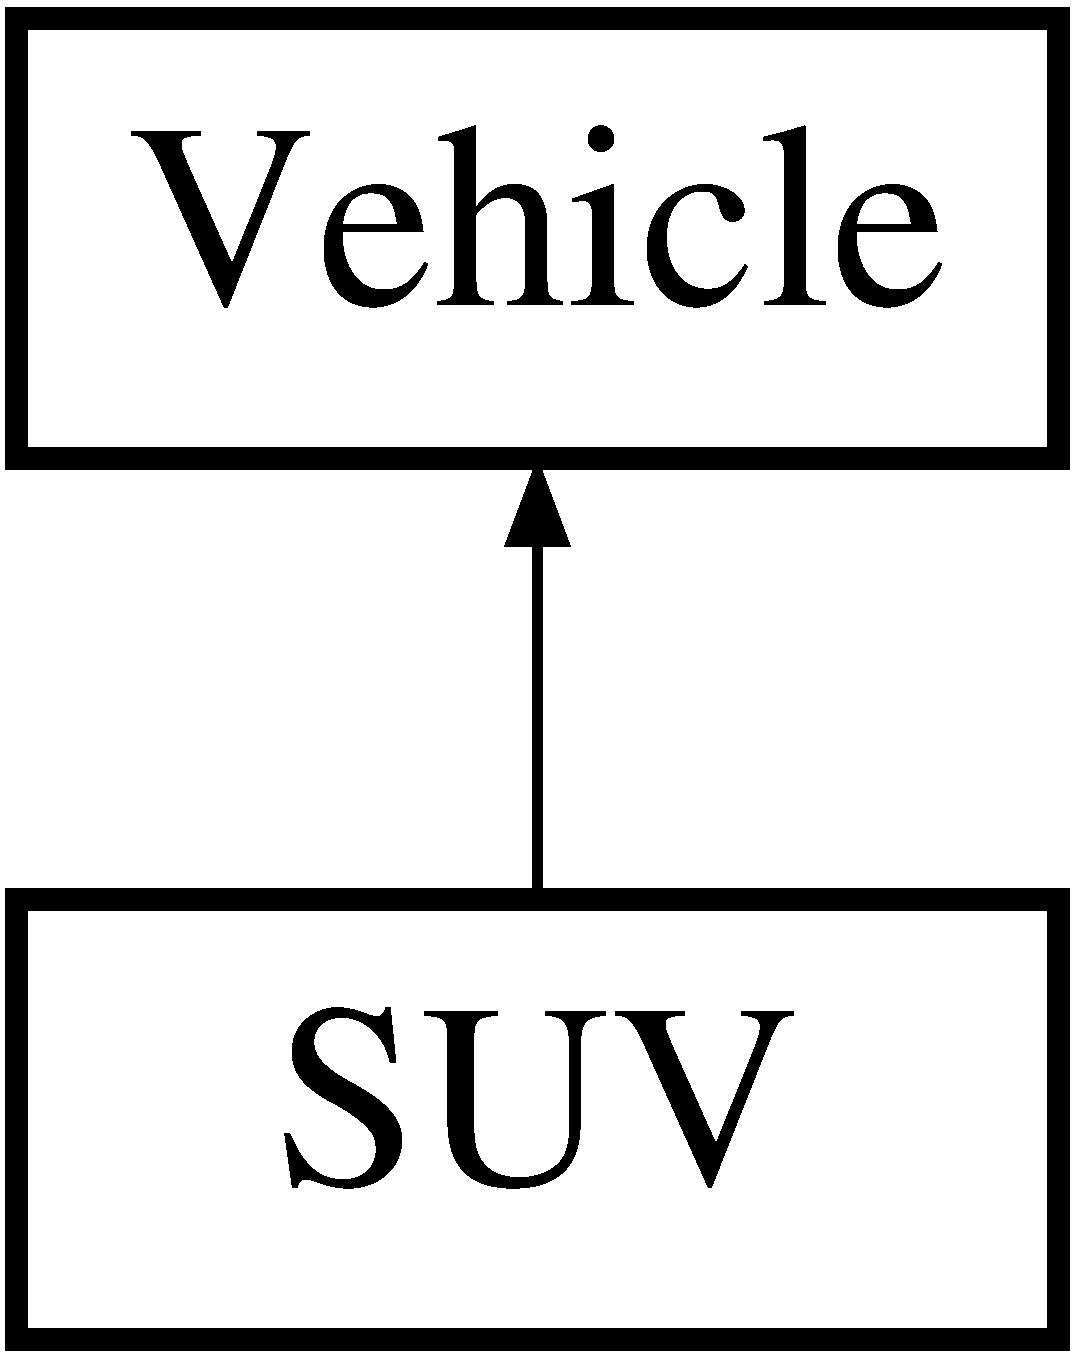
\includegraphics[height=2.000000cm]{class_s_u_v}
\end{center}
\end{figure}
\subsection*{Public Member Functions}
\begin{DoxyCompactItemize}
\item 
\hyperlink{class_s_u_v_a146d74592e3be41fd6e2e7a7d05dac0d}{S\+UV} ()
\item 
\hyperlink{class_s_u_v_a221a9726b31f7e69f4e746624d0ea50e}{S\+UV} (string make, string model, int year, string color, int num\+Wheels, int customer\+Num, int status, string type)
\item 
\hyperlink{class_s_u_v_abcf2fe9b86e78678fd634598f4b3c738}{$\sim$\+S\+UV} ()
\end{DoxyCompactItemize}
\subsection*{Additional Inherited Members}


\subsection{Constructor \& Destructor Documentation}
\mbox{\Hypertarget{class_s_u_v_a146d74592e3be41fd6e2e7a7d05dac0d}\label{class_s_u_v_a146d74592e3be41fd6e2e7a7d05dac0d}} 
\index{S\+UV@{S\+UV}!S\+UV@{S\+UV}}
\index{S\+UV@{S\+UV}!S\+UV@{S\+UV}}
\subsubsection{\texorpdfstring{S\+U\+V()}{SUV()}\hspace{0.1cm}{\footnotesize\ttfamily [1/2]}}
{\footnotesize\ttfamily S\+U\+V\+::\+S\+UV (\begin{DoxyParamCaption}{ }\end{DoxyParamCaption})}

\hyperlink{class_s_u_v}{S\+UV} class constructor. \mbox{\Hypertarget{class_s_u_v_a221a9726b31f7e69f4e746624d0ea50e}\label{class_s_u_v_a221a9726b31f7e69f4e746624d0ea50e}} 
\index{S\+UV@{S\+UV}!S\+UV@{S\+UV}}
\index{S\+UV@{S\+UV}!S\+UV@{S\+UV}}
\subsubsection{\texorpdfstring{S\+U\+V()}{SUV()}\hspace{0.1cm}{\footnotesize\ttfamily [2/2]}}
{\footnotesize\ttfamily S\+U\+V\+::\+S\+UV (\begin{DoxyParamCaption}\item[{string}]{make,  }\item[{string}]{model,  }\item[{int}]{year,  }\item[{string}]{color,  }\item[{int}]{num\+Wheels,  }\item[{int}]{customer\+ID,  }\item[{int}]{status,  }\item[{string}]{type }\end{DoxyParamCaption})}

\hyperlink{class_s_u_v}{S\+UV} class constructor takes in several parameters that apply to a \hyperlink{class_s_u_v}{S\+UV} object. \mbox{\Hypertarget{class_s_u_v_abcf2fe9b86e78678fd634598f4b3c738}\label{class_s_u_v_abcf2fe9b86e78678fd634598f4b3c738}} 
\index{S\+UV@{S\+UV}!````~S\+UV@{$\sim$\+S\+UV}}
\index{````~S\+UV@{$\sim$\+S\+UV}!S\+UV@{S\+UV}}
\subsubsection{\texorpdfstring{$\sim$\+S\+U\+V()}{~SUV()}}
{\footnotesize\ttfamily S\+U\+V\+::$\sim$\+S\+UV (\begin{DoxyParamCaption}{ }\end{DoxyParamCaption})}

Destructor 

The documentation for this class was generated from the following files\+:\begin{DoxyCompactItemize}
\item 
\hyperlink{suv_8h}{suv.\+h}\item 
\hyperlink{suv_8cpp}{suv.\+cpp}\end{DoxyCompactItemize}

\hypertarget{class_truck}{}\section{Truck Class Reference}
\label{class_truck}\index{Truck@{Truck}}
Inheritance diagram for Truck\+:\begin{figure}[H]
\begin{center}
\leavevmode
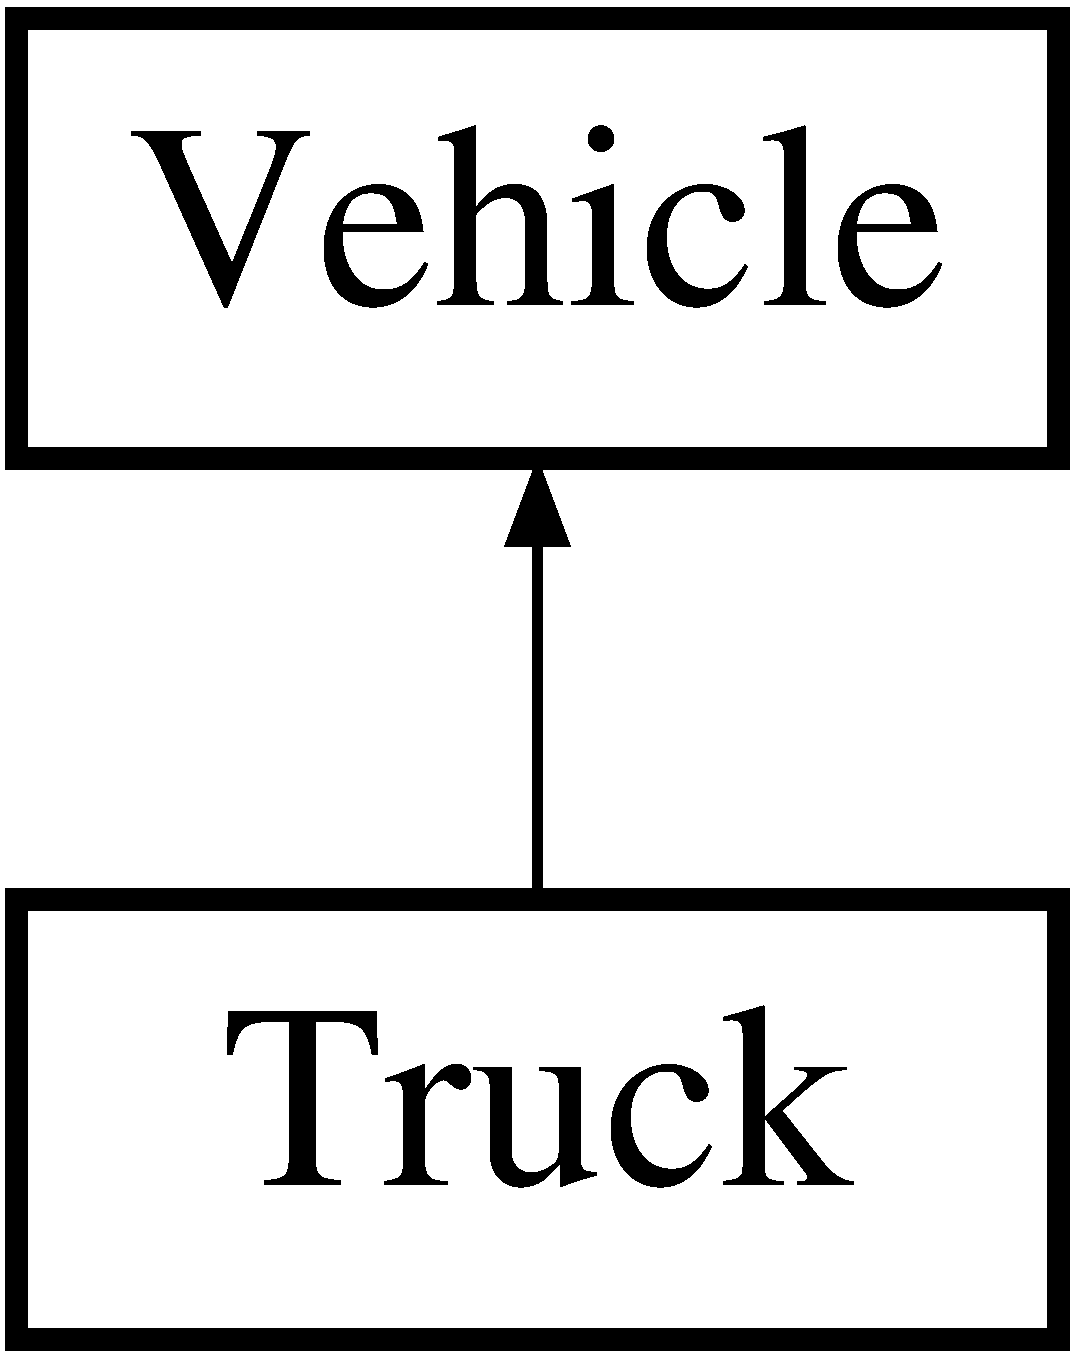
\includegraphics[height=2.000000cm]{class_truck}
\end{center}
\end{figure}
\subsection*{Public Member Functions}
\begin{DoxyCompactItemize}
\item 
\hyperlink{class_truck_a87e358bca8fe34e6299c6ff233afb08b}{Truck} ()
\item 
\hyperlink{class_truck_a134acf4a22664f65be38ba2843b2ae18}{Truck} (string make, string model, int year, string color, int num\+Wheels, int customer\+Num, int status, string type)
\item 
\hyperlink{class_truck_afe887186d0490451a8ce4a3ef433dee3}{$\sim$\+Truck} ()
\end{DoxyCompactItemize}
\subsection*{Additional Inherited Members}


\subsection{Constructor \& Destructor Documentation}
\mbox{\Hypertarget{class_truck_a87e358bca8fe34e6299c6ff233afb08b}\label{class_truck_a87e358bca8fe34e6299c6ff233afb08b}} 
\index{Truck@{Truck}!Truck@{Truck}}
\index{Truck@{Truck}!Truck@{Truck}}
\subsubsection{\texorpdfstring{Truck()}{Truck()}\hspace{0.1cm}{\footnotesize\ttfamily [1/2]}}
{\footnotesize\ttfamily Truck\+::\+Truck (\begin{DoxyParamCaption}{ }\end{DoxyParamCaption})}

\hyperlink{class_truck}{Truck} class constructor. \mbox{\Hypertarget{class_truck_a134acf4a22664f65be38ba2843b2ae18}\label{class_truck_a134acf4a22664f65be38ba2843b2ae18}} 
\index{Truck@{Truck}!Truck@{Truck}}
\index{Truck@{Truck}!Truck@{Truck}}
\subsubsection{\texorpdfstring{Truck()}{Truck()}\hspace{0.1cm}{\footnotesize\ttfamily [2/2]}}
{\footnotesize\ttfamily Truck\+::\+Truck (\begin{DoxyParamCaption}\item[{string}]{make,  }\item[{string}]{model,  }\item[{int}]{year,  }\item[{string}]{color,  }\item[{int}]{num\+Wheels,  }\item[{int}]{customer\+ID,  }\item[{int}]{status,  }\item[{string}]{type }\end{DoxyParamCaption})}

\hyperlink{class_truck}{Truck} class constructor takes in several parameters that apply to a \hyperlink{class_truck}{Truck} object. \mbox{\Hypertarget{class_truck_afe887186d0490451a8ce4a3ef433dee3}\label{class_truck_afe887186d0490451a8ce4a3ef433dee3}} 
\index{Truck@{Truck}!````~Truck@{$\sim$\+Truck}}
\index{````~Truck@{$\sim$\+Truck}!Truck@{Truck}}
\subsubsection{\texorpdfstring{$\sim$\+Truck()}{~Truck()}}
{\footnotesize\ttfamily Truck\+::$\sim$\+Truck (\begin{DoxyParamCaption}{ }\end{DoxyParamCaption})}

Destructor 

The documentation for this class was generated from the following files\+:\begin{DoxyCompactItemize}
\item 
\hyperlink{truck_8h}{truck.\+h}\item 
\hyperlink{truck_8cpp}{truck.\+cpp}\end{DoxyCompactItemize}

\hypertarget{class_vehicle}{}\section{Vehicle Class Reference}
\label{class_vehicle}\index{Vehicle@{Vehicle}}
Inheritance diagram for Vehicle\+:\begin{figure}[H]
\begin{center}
\leavevmode
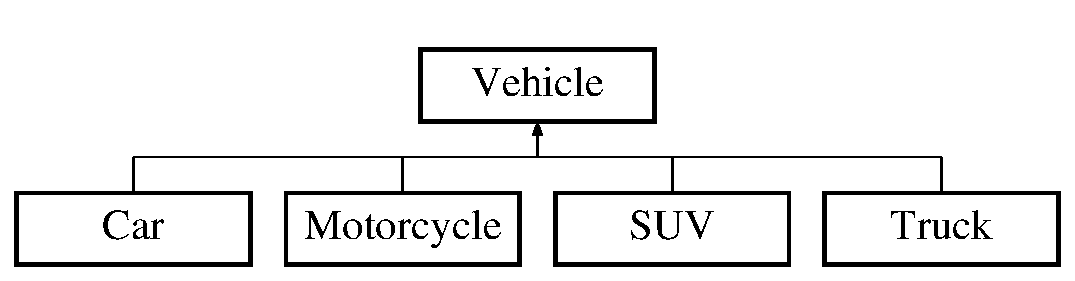
\includegraphics[height=2.000000cm]{class_vehicle}
\end{center}
\end{figure}
\subsection*{Public Member Functions}
\begin{DoxyCompactItemize}
\item 
\hyperlink{class_vehicle_abaad8187d9f2ede4fb8ea18de0a6764c}{Vehicle} ()
\item 
\hyperlink{class_vehicle_a7c366af6337bace71aab2a56bade1b51}{Vehicle} (string make, string model, int year, string color, int num\+Wheels, int customer\+ID, int status, string type)
\item 
\hyperlink{class_vehicle_a61ab140c755b8e0e824d54117cf4546f}{$\sim$\+Vehicle} ()
\item 
void \hyperlink{class_vehicle_a889588751f2751b4c76740407a769ca2}{set\+Make} (string make)
\item 
string \hyperlink{class_vehicle_afc39d455c65b61ffe827127edb92bfc5}{get\+Make} ()
\item 
void \hyperlink{class_vehicle_a3a813eb34cc39eb0790e3b04d2d975e3}{set\+Model} (string model)
\item 
string \hyperlink{class_vehicle_a4ea5cae65802d874f9035f98cafaf51c}{get\+Model} ()
\item 
void \hyperlink{class_vehicle_a8f26a947749fc447adbfb48b3bf5f289}{set\+Year} (int year)
\item 
int \hyperlink{class_vehicle_a206f357a7b9202335f143c1ca3477ef1}{get\+Year} ()
\item 
void \hyperlink{class_vehicle_acdf4eb878866cb43045cd0c62ad808cd}{set\+Color} (string color)
\item 
string \hyperlink{class_vehicle_a94445efb02e754a205520bf39789e031}{get\+Color} ()
\item 
void \hyperlink{class_vehicle_a91f4ad00bfe3d0d330632caf3c1fe77a}{set\+Num\+Wheels} (int num\+Wheels)
\item 
int \hyperlink{class_vehicle_afd8d35a0deef1e846396f90737be9655}{get\+Num\+Wheels} ()
\item 
void \hyperlink{class_vehicle_ab15f9d0d115fa64ec5b3a6c40caca2ff}{set\+Customer\+ID} (int customer\+ID)
\item 
int \hyperlink{class_vehicle_a47dba04c728156ee3e2447cd7d3745c0}{get\+Customer\+ID} ()
\item 
void \hyperlink{class_vehicle_aa547452a11bfd2b20c79b7ee72309a00}{set\+Status} (int status)
\item 
int \hyperlink{class_vehicle_a835b1213216a5821abab0250231f6f2b}{get\+Status} ()
\item 
void \hyperlink{class_vehicle_a053568fb129b4294a82553d68880b07a}{set\+Type} (string type)
\item 
string \hyperlink{class_vehicle_a540c0784a94f351f90011a7e9fee39f0}{get\+Type} ()
\item 
string \hyperlink{class_vehicle_abd9381537867c1a98430ab06ce51898f}{to\+String} ()
\item 
string \hyperlink{class_vehicle_aa614254249eb1f1c0221b782c47d269e}{to\+String\+Rented} ()
\end{DoxyCompactItemize}
\subsection*{Protected Attributes}
\begin{DoxyCompactItemize}
\item 
\mbox{\Hypertarget{class_vehicle_a0f9767be0624891a5416e4734bc90424}\label{class_vehicle_a0f9767be0624891a5416e4734bc90424}} 
string {\bfseries make}
\item 
\mbox{\Hypertarget{class_vehicle_a61799a3b07bd7ad2a07d61af510f91f0}\label{class_vehicle_a61799a3b07bd7ad2a07d61af510f91f0}} 
string {\bfseries model}
\item 
\mbox{\Hypertarget{class_vehicle_ad612fe1e00e266a5d740bb67920211d4}\label{class_vehicle_ad612fe1e00e266a5d740bb67920211d4}} 
int {\bfseries year}
\item 
\mbox{\Hypertarget{class_vehicle_a992c801eab239e432add59c3a8ce5d7e}\label{class_vehicle_a992c801eab239e432add59c3a8ce5d7e}} 
string {\bfseries color}
\item 
\mbox{\Hypertarget{class_vehicle_a08e3dd6521f07827a8c0e6c509f61b7c}\label{class_vehicle_a08e3dd6521f07827a8c0e6c509f61b7c}} 
int {\bfseries num\+Wheels}
\item 
\mbox{\Hypertarget{class_vehicle_af4ac7afd3bab1519a1b5f247c44bde5b}\label{class_vehicle_af4ac7afd3bab1519a1b5f247c44bde5b}} 
int {\bfseries customer\+ID}
\item 
\mbox{\Hypertarget{class_vehicle_a684a4340e817cdefcde3b0d9d1b98f4c}\label{class_vehicle_a684a4340e817cdefcde3b0d9d1b98f4c}} 
int {\bfseries status}
\item 
\mbox{\Hypertarget{class_vehicle_a99487b9f05bb36855d7af79df4f60781}\label{class_vehicle_a99487b9f05bb36855d7af79df4f60781}} 
string {\bfseries type}
\end{DoxyCompactItemize}


\subsection{Constructor \& Destructor Documentation}
\mbox{\Hypertarget{class_vehicle_abaad8187d9f2ede4fb8ea18de0a6764c}\label{class_vehicle_abaad8187d9f2ede4fb8ea18de0a6764c}} 
\index{Vehicle@{Vehicle}!Vehicle@{Vehicle}}
\index{Vehicle@{Vehicle}!Vehicle@{Vehicle}}
\subsubsection{\texorpdfstring{Vehicle()}{Vehicle()}\hspace{0.1cm}{\footnotesize\ttfamily [1/2]}}
{\footnotesize\ttfamily Vehicle\+::\+Vehicle (\begin{DoxyParamCaption}{ }\end{DoxyParamCaption})}

\hyperlink{class_vehicle}{Vehicle} class constructor. \mbox{\Hypertarget{class_vehicle_a7c366af6337bace71aab2a56bade1b51}\label{class_vehicle_a7c366af6337bace71aab2a56bade1b51}} 
\index{Vehicle@{Vehicle}!Vehicle@{Vehicle}}
\index{Vehicle@{Vehicle}!Vehicle@{Vehicle}}
\subsubsection{\texorpdfstring{Vehicle()}{Vehicle()}\hspace{0.1cm}{\footnotesize\ttfamily [2/2]}}
{\footnotesize\ttfamily Vehicle\+::\+Vehicle (\begin{DoxyParamCaption}\item[{string}]{make,  }\item[{string}]{model,  }\item[{int}]{year,  }\item[{string}]{color,  }\item[{int}]{num\+Wheels,  }\item[{int}]{customer\+ID,  }\item[{int}]{status,  }\item[{string}]{type }\end{DoxyParamCaption})}

\hyperlink{class_vehicle}{Vehicle} class constructor takes in several parameters that apply to a \hyperlink{class_vehicle}{Vehicle} object. 
\begin{DoxyParams}{Parameters}
{\em make} & manufacturer of vehicle \\
\hline
{\em model} & variation of vehicle \\
\hline
{\em year} & when vehicle started to be in production \\
\hline
{\em color} & color of vehicle \\
\hline
{\em num\+Wheels} & number of wheels \\
\hline
{\em customer\+ID} & identification of customer object \\
\hline
{\em status} & current state of vehicle object \\
\hline
{\em type} & the type of vehicle M, C, or T \\
\hline
\end{DoxyParams}
\mbox{\Hypertarget{class_vehicle_a61ab140c755b8e0e824d54117cf4546f}\label{class_vehicle_a61ab140c755b8e0e824d54117cf4546f}} 
\index{Vehicle@{Vehicle}!````~Vehicle@{$\sim$\+Vehicle}}
\index{````~Vehicle@{$\sim$\+Vehicle}!Vehicle@{Vehicle}}
\subsubsection{\texorpdfstring{$\sim$\+Vehicle()}{~Vehicle()}}
{\footnotesize\ttfamily Vehicle\+::$\sim$\+Vehicle (\begin{DoxyParamCaption}{ }\end{DoxyParamCaption})}

Destructor 

\subsection{Member Function Documentation}
\mbox{\Hypertarget{class_vehicle_a94445efb02e754a205520bf39789e031}\label{class_vehicle_a94445efb02e754a205520bf39789e031}} 
\index{Vehicle@{Vehicle}!get\+Color@{get\+Color}}
\index{get\+Color@{get\+Color}!Vehicle@{Vehicle}}
\subsubsection{\texorpdfstring{get\+Color()}{getColor()}}
{\footnotesize\ttfamily string Vehicle\+::get\+Color (\begin{DoxyParamCaption}{ }\end{DoxyParamCaption})}

Fucntion returns the color of \hyperlink{class_vehicle}{Vehicle}. \begin{DoxyReturn}{Returns}
color 
\end{DoxyReturn}
\mbox{\Hypertarget{class_vehicle_a47dba04c728156ee3e2447cd7d3745c0}\label{class_vehicle_a47dba04c728156ee3e2447cd7d3745c0}} 
\index{Vehicle@{Vehicle}!get\+Customer\+ID@{get\+Customer\+ID}}
\index{get\+Customer\+ID@{get\+Customer\+ID}!Vehicle@{Vehicle}}
\subsubsection{\texorpdfstring{get\+Customer\+I\+D()}{getCustomerID()}}
{\footnotesize\ttfamily int Vehicle\+::get\+Customer\+ID (\begin{DoxyParamCaption}{ }\end{DoxyParamCaption})}

Fucntion returns the customer\+ID of \hyperlink{class_customer}{Customer}. \begin{DoxyReturn}{Returns}
customer\+ID 
\end{DoxyReturn}
\mbox{\Hypertarget{class_vehicle_afc39d455c65b61ffe827127edb92bfc5}\label{class_vehicle_afc39d455c65b61ffe827127edb92bfc5}} 
\index{Vehicle@{Vehicle}!get\+Make@{get\+Make}}
\index{get\+Make@{get\+Make}!Vehicle@{Vehicle}}
\subsubsection{\texorpdfstring{get\+Make()}{getMake()}}
{\footnotesize\ttfamily string Vehicle\+::get\+Make (\begin{DoxyParamCaption}{ }\end{DoxyParamCaption})}

Fucntion returns the make of \hyperlink{class_vehicle}{Vehicle}. \begin{DoxyReturn}{Returns}
make 
\end{DoxyReturn}
\mbox{\Hypertarget{class_vehicle_a4ea5cae65802d874f9035f98cafaf51c}\label{class_vehicle_a4ea5cae65802d874f9035f98cafaf51c}} 
\index{Vehicle@{Vehicle}!get\+Model@{get\+Model}}
\index{get\+Model@{get\+Model}!Vehicle@{Vehicle}}
\subsubsection{\texorpdfstring{get\+Model()}{getModel()}}
{\footnotesize\ttfamily string Vehicle\+::get\+Model (\begin{DoxyParamCaption}{ }\end{DoxyParamCaption})}

Fucntion returns the model of \hyperlink{class_vehicle}{Vehicle}. \begin{DoxyReturn}{Returns}
model 
\end{DoxyReturn}
\mbox{\Hypertarget{class_vehicle_afd8d35a0deef1e846396f90737be9655}\label{class_vehicle_afd8d35a0deef1e846396f90737be9655}} 
\index{Vehicle@{Vehicle}!get\+Num\+Wheels@{get\+Num\+Wheels}}
\index{get\+Num\+Wheels@{get\+Num\+Wheels}!Vehicle@{Vehicle}}
\subsubsection{\texorpdfstring{get\+Num\+Wheels()}{getNumWheels()}}
{\footnotesize\ttfamily int Vehicle\+::get\+Num\+Wheels (\begin{DoxyParamCaption}{ }\end{DoxyParamCaption})}

Fucntion returns the number of wheels of a \hyperlink{class_vehicle}{Vehicle}. \begin{DoxyReturn}{Returns}
num\+Wheels 
\end{DoxyReturn}
\mbox{\Hypertarget{class_vehicle_a835b1213216a5821abab0250231f6f2b}\label{class_vehicle_a835b1213216a5821abab0250231f6f2b}} 
\index{Vehicle@{Vehicle}!get\+Status@{get\+Status}}
\index{get\+Status@{get\+Status}!Vehicle@{Vehicle}}
\subsubsection{\texorpdfstring{get\+Status()}{getStatus()}}
{\footnotesize\ttfamily int Vehicle\+::get\+Status (\begin{DoxyParamCaption}{ }\end{DoxyParamCaption})}

Fucntion returns the status of \hyperlink{class_vehicle}{Vehicle}. \begin{DoxyReturn}{Returns}
status 
\end{DoxyReturn}
\mbox{\Hypertarget{class_vehicle_a540c0784a94f351f90011a7e9fee39f0}\label{class_vehicle_a540c0784a94f351f90011a7e9fee39f0}} 
\index{Vehicle@{Vehicle}!get\+Type@{get\+Type}}
\index{get\+Type@{get\+Type}!Vehicle@{Vehicle}}
\subsubsection{\texorpdfstring{get\+Type()}{getType()}}
{\footnotesize\ttfamily string Vehicle\+::get\+Type (\begin{DoxyParamCaption}{ }\end{DoxyParamCaption})}

Fucntion returns the type of \hyperlink{class_vehicle}{Vehicle}. \begin{DoxyReturn}{Returns}
type 
\end{DoxyReturn}
\mbox{\Hypertarget{class_vehicle_a206f357a7b9202335f143c1ca3477ef1}\label{class_vehicle_a206f357a7b9202335f143c1ca3477ef1}} 
\index{Vehicle@{Vehicle}!get\+Year@{get\+Year}}
\index{get\+Year@{get\+Year}!Vehicle@{Vehicle}}
\subsubsection{\texorpdfstring{get\+Year()}{getYear()}}
{\footnotesize\ttfamily int Vehicle\+::get\+Year (\begin{DoxyParamCaption}{ }\end{DoxyParamCaption})}

Fucntion returns the year of \hyperlink{class_vehicle}{Vehicle}. \begin{DoxyReturn}{Returns}
year 
\end{DoxyReturn}
\mbox{\Hypertarget{class_vehicle_acdf4eb878866cb43045cd0c62ad808cd}\label{class_vehicle_acdf4eb878866cb43045cd0c62ad808cd}} 
\index{Vehicle@{Vehicle}!set\+Color@{set\+Color}}
\index{set\+Color@{set\+Color}!Vehicle@{Vehicle}}
\subsubsection{\texorpdfstring{set\+Color()}{setColor()}}
{\footnotesize\ttfamily void Vehicle\+::set\+Color (\begin{DoxyParamCaption}\item[{string}]{color }\end{DoxyParamCaption})}

Function populates color with string. 
\begin{DoxyParams}{Parameters}
{\em color} & \\
\hline
\end{DoxyParams}
\begin{DoxyReturn}{Returns}
none 
\end{DoxyReturn}
\mbox{\Hypertarget{class_vehicle_ab15f9d0d115fa64ec5b3a6c40caca2ff}\label{class_vehicle_ab15f9d0d115fa64ec5b3a6c40caca2ff}} 
\index{Vehicle@{Vehicle}!set\+Customer\+ID@{set\+Customer\+ID}}
\index{set\+Customer\+ID@{set\+Customer\+ID}!Vehicle@{Vehicle}}
\subsubsection{\texorpdfstring{set\+Customer\+I\+D()}{setCustomerID()}}
{\footnotesize\ttfamily void Vehicle\+::set\+Customer\+ID (\begin{DoxyParamCaption}\item[{int}]{customer\+ID }\end{DoxyParamCaption})}

Function populates customer\+ID with string. 
\begin{DoxyParams}{Parameters}
{\em customer\+ID} & \\
\hline
\end{DoxyParams}
\begin{DoxyReturn}{Returns}
none 
\end{DoxyReturn}
\mbox{\Hypertarget{class_vehicle_a889588751f2751b4c76740407a769ca2}\label{class_vehicle_a889588751f2751b4c76740407a769ca2}} 
\index{Vehicle@{Vehicle}!set\+Make@{set\+Make}}
\index{set\+Make@{set\+Make}!Vehicle@{Vehicle}}
\subsubsection{\texorpdfstring{set\+Make()}{setMake()}}
{\footnotesize\ttfamily void Vehicle\+::set\+Make (\begin{DoxyParamCaption}\item[{string}]{make }\end{DoxyParamCaption})}

Function populates make with string. 
\begin{DoxyParams}{Parameters}
{\em make} & \\
\hline
\end{DoxyParams}
\begin{DoxyReturn}{Returns}
none 
\end{DoxyReturn}
\mbox{\Hypertarget{class_vehicle_a3a813eb34cc39eb0790e3b04d2d975e3}\label{class_vehicle_a3a813eb34cc39eb0790e3b04d2d975e3}} 
\index{Vehicle@{Vehicle}!set\+Model@{set\+Model}}
\index{set\+Model@{set\+Model}!Vehicle@{Vehicle}}
\subsubsection{\texorpdfstring{set\+Model()}{setModel()}}
{\footnotesize\ttfamily void Vehicle\+::set\+Model (\begin{DoxyParamCaption}\item[{string}]{model }\end{DoxyParamCaption})}

Function populates model with string. 
\begin{DoxyParams}{Parameters}
{\em model} & \\
\hline
\end{DoxyParams}
\begin{DoxyReturn}{Returns}
none 
\end{DoxyReturn}
\mbox{\Hypertarget{class_vehicle_a91f4ad00bfe3d0d330632caf3c1fe77a}\label{class_vehicle_a91f4ad00bfe3d0d330632caf3c1fe77a}} 
\index{Vehicle@{Vehicle}!set\+Num\+Wheels@{set\+Num\+Wheels}}
\index{set\+Num\+Wheels@{set\+Num\+Wheels}!Vehicle@{Vehicle}}
\subsubsection{\texorpdfstring{set\+Num\+Wheels()}{setNumWheels()}}
{\footnotesize\ttfamily void Vehicle\+::set\+Num\+Wheels (\begin{DoxyParamCaption}\item[{int}]{num\+Wheels }\end{DoxyParamCaption})}

Function populates num\+Wheels with string. 
\begin{DoxyParams}{Parameters}
{\em num\+Wheels} & \\
\hline
\end{DoxyParams}
\begin{DoxyReturn}{Returns}
none 
\end{DoxyReturn}
\mbox{\Hypertarget{class_vehicle_aa547452a11bfd2b20c79b7ee72309a00}\label{class_vehicle_aa547452a11bfd2b20c79b7ee72309a00}} 
\index{Vehicle@{Vehicle}!set\+Status@{set\+Status}}
\index{set\+Status@{set\+Status}!Vehicle@{Vehicle}}
\subsubsection{\texorpdfstring{set\+Status()}{setStatus()}}
{\footnotesize\ttfamily void Vehicle\+::set\+Status (\begin{DoxyParamCaption}\item[{int}]{status }\end{DoxyParamCaption})}

Function populates status with string. 
\begin{DoxyParams}{Parameters}
{\em status} & \\
\hline
\end{DoxyParams}
\begin{DoxyReturn}{Returns}
none 
\end{DoxyReturn}
\mbox{\Hypertarget{class_vehicle_a053568fb129b4294a82553d68880b07a}\label{class_vehicle_a053568fb129b4294a82553d68880b07a}} 
\index{Vehicle@{Vehicle}!set\+Type@{set\+Type}}
\index{set\+Type@{set\+Type}!Vehicle@{Vehicle}}
\subsubsection{\texorpdfstring{set\+Type()}{setType()}}
{\footnotesize\ttfamily void Vehicle\+::set\+Type (\begin{DoxyParamCaption}\item[{string}]{type }\end{DoxyParamCaption})}

Function populates type with string. 
\begin{DoxyParams}{Parameters}
{\em type} & \\
\hline
\end{DoxyParams}
\begin{DoxyReturn}{Returns}
none 
\end{DoxyReturn}
\mbox{\Hypertarget{class_vehicle_a8f26a947749fc447adbfb48b3bf5f289}\label{class_vehicle_a8f26a947749fc447adbfb48b3bf5f289}} 
\index{Vehicle@{Vehicle}!set\+Year@{set\+Year}}
\index{set\+Year@{set\+Year}!Vehicle@{Vehicle}}
\subsubsection{\texorpdfstring{set\+Year()}{setYear()}}
{\footnotesize\ttfamily void Vehicle\+::set\+Year (\begin{DoxyParamCaption}\item[{int}]{year }\end{DoxyParamCaption})}

Function populates year with string. 
\begin{DoxyParams}{Parameters}
{\em year} & \\
\hline
\end{DoxyParams}
\begin{DoxyReturn}{Returns}
none 
\end{DoxyReturn}
\mbox{\Hypertarget{class_vehicle_abd9381537867c1a98430ab06ce51898f}\label{class_vehicle_abd9381537867c1a98430ab06ce51898f}} 
\index{Vehicle@{Vehicle}!to\+String@{to\+String}}
\index{to\+String@{to\+String}!Vehicle@{Vehicle}}
\subsubsection{\texorpdfstring{to\+String()}{toString()}}
{\footnotesize\ttfamily string Vehicle\+::to\+String (\begin{DoxyParamCaption}{ }\end{DoxyParamCaption})}

Fucntion returns a string formated to \char`\"{}make model year color type\char`\"{} \mbox{\Hypertarget{class_vehicle_aa614254249eb1f1c0221b782c47d269e}\label{class_vehicle_aa614254249eb1f1c0221b782c47d269e}} 
\index{Vehicle@{Vehicle}!to\+String\+Rented@{to\+String\+Rented}}
\index{to\+String\+Rented@{to\+String\+Rented}!Vehicle@{Vehicle}}
\subsubsection{\texorpdfstring{to\+String\+Rented()}{toStringRented()}}
{\footnotesize\ttfamily string Vehicle\+::to\+String\+Rented (\begin{DoxyParamCaption}{ }\end{DoxyParamCaption})}

Fucntion returns a string formated to \char`\"{}make model year color type\char`\"{} 

The documentation for this class was generated from the following files\+:\begin{DoxyCompactItemize}
\item 
\hyperlink{vehicle_8h}{vehicle.\+h}\item 
\hyperlink{vehicle_8cpp}{vehicle.\+cpp}\end{DoxyCompactItemize}

\chapter{File Documentation}
\hypertarget{car_8cpp}{}\section{car.\+cpp File Reference}
\label{car_8cpp}\index{car.\+cpp@{car.\+cpp}}


I\+T\+CS 3112 Rent-\/\+A-\/\+Ride Final Project.  


{\ttfamily \#include $<$iostream$>$}\newline
{\ttfamily \#include $<$fstream$>$}\newline
{\ttfamily \#include $<$string$>$}\newline
{\ttfamily \#include \char`\"{}car.\+h\char`\"{}}\newline


\subsection{Detailed Description}
I\+T\+CS 3112 Rent-\/\+A-\/\+Ride Final Project. 

\begin{DoxyAuthor}{Author}
John Poulos, jpoulos2 
\end{DoxyAuthor}
\begin{DoxyDate}{Date}
Oct 16, 2017
\end{DoxyDate}
\hypertarget{vehicle_8h_DESCRIPTION}{}\subsection{D\+E\+S\+C\+R\+I\+P\+T\+I\+ON}\label{vehicle_8h_DESCRIPTION}
Implementation file for car. 
\hypertarget{car_8h}{}\section{car.\+h File Reference}
\label{car_8h}\index{car.\+h@{car.\+h}}


I\+T\+CS 3112 Rent-\/\+A-\/\+Ride Final Project.  


{\ttfamily \#include \char`\"{}vehicle.\+h\char`\"{}}\newline
{\ttfamily \#include $<$iostream$>$}\newline
{\ttfamily \#include $<$fstream$>$}\newline
{\ttfamily \#include $<$string$>$}\newline
\subsection*{Classes}
\begin{DoxyCompactItemize}
\item 
class \hyperlink{class_car}{Car}
\end{DoxyCompactItemize}


\subsection{Detailed Description}
I\+T\+CS 3112 Rent-\/\+A-\/\+Ride Final Project. 

\begin{DoxyAuthor}{Author}
John Poulos, jpoulos2 
\end{DoxyAuthor}
\begin{DoxyDate}{Date}
Oct 16, 2017
\end{DoxyDate}
\hypertarget{vehicle_8h_DESCRIPTION}{}\subsection{D\+E\+S\+C\+R\+I\+P\+T\+I\+ON}\label{vehicle_8h_DESCRIPTION}
Header file for the car object. 
\hypertarget{customer_8h}{}\section{customer.\+h File Reference}
\label{customer_8h}\index{customer.\+h@{customer.\+h}}


I\+T\+CS 3112 Final Project.  


{\ttfamily \#include $<$iostream$>$}\newline
{\ttfamily \#include $<$string$>$}\newline
\subsection*{Classes}
\begin{DoxyCompactItemize}
\item 
class \hyperlink{class_customer}{Customer}
\end{DoxyCompactItemize}


\subsection{Detailed Description}
I\+T\+CS 3112 Final Project. 

\begin{DoxyAuthor}{Author}
John Poulos, jpoulos2 
\end{DoxyAuthor}
\begin{DoxyDate}{Date}
Dec 2, 2017
\end{DoxyDate}
\hypertarget{vehicle_8h_DESCRIPTION}{}\subsection{D\+E\+S\+C\+R\+I\+P\+T\+I\+ON}\label{vehicle_8h_DESCRIPTION}
Header file for \hyperlink{class_customer}{Customer} definitions. 
\hypertarget{motorcycle_8cpp}{}\section{motorcycle.\+cpp File Reference}
\label{motorcycle_8cpp}\index{motorcycle.\+cpp@{motorcycle.\+cpp}}


I\+T\+CS 3112 Rent-\/\+A-\/\+Ride Final Project.  


{\ttfamily \#include $<$iostream$>$}\newline
{\ttfamily \#include $<$fstream$>$}\newline
{\ttfamily \#include $<$string$>$}\newline
{\ttfamily \#include \char`\"{}motorcycle.\+h\char`\"{}}\newline


\subsection{Detailed Description}
I\+T\+CS 3112 Rent-\/\+A-\/\+Ride Final Project. 

\begin{DoxyAuthor}{Author}
John Poulos, jpoulos2 
\end{DoxyAuthor}
\begin{DoxyDate}{Date}
Oct 16, 2017
\end{DoxyDate}
\hypertarget{vehicle_8h_DESCRIPTION}{}\subsection{D\+E\+S\+C\+R\+I\+P\+T\+I\+ON}\label{vehicle_8h_DESCRIPTION}
Implementation file for \hyperlink{class_motorcycle}{Motorcycle}, child of \hyperlink{car_8cpp}{car.\+cpp}. 
\hypertarget{motorcycle_8h}{}\section{motorcycle.\+h File Reference}
\label{motorcycle_8h}\index{motorcycle.\+h@{motorcycle.\+h}}


I\+T\+CS 3112 Rent-\/\+A-\/\+Ride Final Project.  


{\ttfamily \#include \char`\"{}vehicle.\+h\char`\"{}}\newline
{\ttfamily \#include $<$iostream$>$}\newline
{\ttfamily \#include $<$fstream$>$}\newline
{\ttfamily \#include $<$string$>$}\newline
\subsection*{Classes}
\begin{DoxyCompactItemize}
\item 
class \hyperlink{class_motorcycle}{Motorcycle}
\end{DoxyCompactItemize}


\subsection{Detailed Description}
I\+T\+CS 3112 Rent-\/\+A-\/\+Ride Final Project. 

\begin{DoxyAuthor}{Author}
John Poulos, jpoulos2 
\end{DoxyAuthor}
\begin{DoxyDate}{Date}
Oct 16, 2017
\end{DoxyDate}
\hypertarget{vehicle_8h_DESCRIPTION}{}\subsection{D\+E\+S\+C\+R\+I\+P\+T\+I\+ON}\label{vehicle_8h_DESCRIPTION}
Header file for the \hyperlink{class_motorcycle}{Motorcycle} object. 
\hypertarget{_ra_r_g_u_i_8cpp}{}\section{Ra\+R\+G\+U\+I.\+cpp File Reference}
\label{_ra_r_g_u_i_8cpp}\index{Ra\+R\+G\+U\+I.\+cpp@{Ra\+R\+G\+U\+I.\+cpp}}


I\+T\+CS 3112 Rent-\/\+A-\/\+Ride Final Project.  


{\ttfamily \#include $<$F\+L/\+Fl.\+H$>$}\newline
{\ttfamily \#include $<$F\+L/\+Fl\+\_\+\+Double\+\_\+\+Window.\+H$>$}\newline
{\ttfamily \#include $<$F\+L/\+Fl\+\_\+\+Browser.\+H$>$}\newline
{\ttfamily \#include $<$F\+L/\+Fl\+\_\+\+Hold\+\_\+\+Browser.\+H$>$}\newline
{\ttfamily \#include $<$F\+L/\+Fl\+\_\+\+Input.\+H$>$}\newline
{\ttfamily \#include $<$F\+L/\+Fl\+\_\+\+Output.\+H$>$}\newline
{\ttfamily \#include $<$F\+L/\+Fl\+\_\+\+Table.\+H$>$}\newline
{\ttfamily \#include $<$F\+L/\+Fl\+\_\+\+Button.\+H$>$}\newline
{\ttfamily \#include $<$F\+L/fl\+\_\+draw.\+H$>$}\newline
{\ttfamily \#include $<$F\+L/\+Fl\+\_\+\+Widget.\+H$>$}\newline
{\ttfamily \#include $<$F\+L/\+Fl\+\_\+\+Choice.\+H$>$}\newline
{\ttfamily \#include $<$F\+L/fl\+\_\+ask.\+H$>$}\newline
{\ttfamily \#include $<$stdlib.\+h$>$}\newline
{\ttfamily \#include $<$iostream$>$}\newline
{\ttfamily \#include $<$string$>$}\newline
{\ttfamily \#include $<$stdio.\+h$>$}\newline
{\ttfamily \#include $<$vector$>$}\newline
{\ttfamily \#include $<$sstream$>$}\newline
{\ttfamily \#include \char`\"{}car.\+h\char`\"{}}\newline
{\ttfamily \#include \char`\"{}truck.\+h\char`\"{}}\newline
{\ttfamily \#include \char`\"{}suv.\+h\char`\"{}}\newline
{\ttfamily \#include \char`\"{}motorcycle.\+h\char`\"{}}\newline
{\ttfamily \#include \char`\"{}customer.\+h\char`\"{}}\newline
{\ttfamily \#include \char`\"{}rental\+Manager.\+h\char`\"{}}\newline
\subsection*{Functions}
\begin{DoxyCompactItemize}
\item 
Fl\+\_\+\+Double\+\_\+\+Window \hyperlink{_ra_r_g_u_i_8cpp_a33b64c7cf3f1bc66abe4eaafea28726e}{win} (1500, 700, \char`\"{}Rent-\/A-\/Ride\char`\"{})
\item 
Fl\+\_\+\+Hold\+\_\+\+Browser \hyperlink{_ra_r_g_u_i_8cpp_aa3c4a2d1a0d5026bc0d74a8e9ed4a2c3}{customer\+View} (40, 80, 200, 200,\char`\"{}Customers\char`\"{})
\item 
Fl\+\_\+\+Hold\+\_\+\+Browser \hyperlink{_ra_r_g_u_i_8cpp_ab07c2f2b9a395e63eec3e3c0fae7c0a8}{avail} (280, 80, 225, 200,\char`\"{}Available Vehicles\char`\"{})
\item 
Fl\+\_\+\+Hold\+\_\+\+Browser \hyperlink{_ra_r_g_u_i_8cpp_a74ccc960aca210a58a3e86b2e6dc75d8}{rent} (545, 80, 270, 200,\char`\"{}Rent\char`\"{})
\item 
Fl\+\_\+\+Hold\+\_\+\+Browser \hyperlink{_ra_r_g_u_i_8cpp_a1d5c803b3f82157eb10d9e3b39b45fed}{detail} (855, 80, 240, 200,\char`\"{}Out for detail\char`\"{})
\item 
Fl\+\_\+\+Hold\+\_\+\+Browser \hyperlink{_ra_r_g_u_i_8cpp_a28f722a1c103719a068d6b34b7ecec5e}{repair} (1135, 80, 240, 200,\char`\"{}Out for repair\char`\"{})
\item 
\mbox{\Hypertarget{_ra_r_g_u_i_8cpp_a01b79528f8f713340097c5f4bc78156f}\label{_ra_r_g_u_i_8cpp_a01b79528f8f713340097c5f4bc78156f}} 
Fl\+\_\+\+Button {\bfseries rent\+Vehicle} (40, 300, 200, 30,\char`\"{}Rent vehicle\char`\"{})
\item 
\mbox{\Hypertarget{_ra_r_g_u_i_8cpp_ac1b712d69a4e6d57f5519dda3863f9db}\label{_ra_r_g_u_i_8cpp_ac1b712d69a4e6d57f5519dda3863f9db}} 
Fl\+\_\+\+Button {\bfseries return\+Vehicle} (280, 300, 225, 30,\char`\"{}Return vehicle\char`\"{})
\item 
\mbox{\Hypertarget{_ra_r_g_u_i_8cpp_a0c4000d514fab9af974e8e8909ea1598}\label{_ra_r_g_u_i_8cpp_a0c4000d514fab9af974e8e8909ea1598}} 
Fl\+\_\+\+Button {\bfseries return\+Vehicle\+Problem} (545, 300, 270, 30,\char`\"{}Return \hyperlink{class_vehicle}{Vehicle} (With problem)\char`\"{})
\item 
\mbox{\Hypertarget{_ra_r_g_u_i_8cpp_a66a636bb5678a70cb5cd54071a1b5a74}\label{_ra_r_g_u_i_8cpp_a66a636bb5678a70cb5cd54071a1b5a74}} 
Fl\+\_\+\+Button {\bfseries repair\+Vehicle} (1135, 300, 240, 30,\char`\"{}Repair vehicle\char`\"{})
\item 
\mbox{\Hypertarget{_ra_r_g_u_i_8cpp_a137ba323401e4e81322c77a00719d23b}\label{_ra_r_g_u_i_8cpp_a137ba323401e4e81322c77a00719d23b}} 
Fl\+\_\+\+Button {\bfseries detail\+Vehicle} (855, 300, 240, 30,\char`\"{}Detail vehicle\char`\"{})
\item 
\mbox{\Hypertarget{_ra_r_g_u_i_8cpp_a63379b93f2a988d903b9d1579ba3f80a}\label{_ra_r_g_u_i_8cpp_a63379b93f2a988d903b9d1579ba3f80a}} 
Fl\+\_\+\+Input {\bfseries person\+Name} (100, 400, 300, 30,\char`\"{}First Name\char`\"{})
\item 
\mbox{\Hypertarget{_ra_r_g_u_i_8cpp_a1de6af9feff9876c53fb47b0752e1c18}\label{_ra_r_g_u_i_8cpp_a1de6af9feff9876c53fb47b0752e1c18}} 
Fl\+\_\+\+Input {\bfseries person\+Last\+Name} (100, 450, 300, 30,\char`\"{}Last Name\char`\"{})
\item 
\mbox{\Hypertarget{_ra_r_g_u_i_8cpp_ac109fdfc648b844e81f4c64aed258145}\label{_ra_r_g_u_i_8cpp_ac109fdfc648b844e81f4c64aed258145}} 
Fl\+\_\+\+Button {\bfseries add\+Customer} (100, 500, 300, 30,\char`\"{}Add customer\char`\"{})
\item 
\mbox{\Hypertarget{_ra_r_g_u_i_8cpp_a8b1f3fb9849face95e4113c6af0f9aaf}\label{_ra_r_g_u_i_8cpp_a8b1f3fb9849face95e4113c6af0f9aaf}} 
Fl\+\_\+\+Input {\bfseries veh\+Make} (600, 400, 200, 30,\char`\"{}Vehicle Make\char`\"{})
\item 
\mbox{\Hypertarget{_ra_r_g_u_i_8cpp_acbf80f51d14e46e7f3bb0b7d2bb37858}\label{_ra_r_g_u_i_8cpp_acbf80f51d14e46e7f3bb0b7d2bb37858}} 
Fl\+\_\+\+Input {\bfseries veh\+Model} (600, 450, 200, 30,\char`\"{}Vehicle Model\char`\"{})
\item 
\mbox{\Hypertarget{_ra_r_g_u_i_8cpp_a0822cc8cc67ce6d996b17a3d03ab423e}\label{_ra_r_g_u_i_8cpp_a0822cc8cc67ce6d996b17a3d03ab423e}} 
Fl\+\_\+\+Input {\bfseries veh\+Year} (600, 500, 200, 30,\char`\"{}Vehicle Year\char`\"{})
\item 
\mbox{\Hypertarget{_ra_r_g_u_i_8cpp_ad399731ae97b69198e4577d9877c05a0}\label{_ra_r_g_u_i_8cpp_ad399731ae97b69198e4577d9877c05a0}} 
Fl\+\_\+\+Choice {\bfseries veh\+Color} (600, 550, 200, 30,\char`\"{}Vehicle Color\char`\"{})
\item 
\mbox{\Hypertarget{_ra_r_g_u_i_8cpp_abe2a518adeb4a1a1bdafc9735543bfbe}\label{_ra_r_g_u_i_8cpp_abe2a518adeb4a1a1bdafc9735543bfbe}} 
Fl\+\_\+\+Choice {\bfseries veh\+Type} (600, 600, 200, 30,\char`\"{}Type\char`\"{})
\item 
\mbox{\Hypertarget{_ra_r_g_u_i_8cpp_aacacb7bf671aa97ac3d6b8f5c836e733}\label{_ra_r_g_u_i_8cpp_aacacb7bf671aa97ac3d6b8f5c836e733}} 
Fl\+\_\+\+Button {\bfseries add\+Vehicle} (600, 650, 200, 30,\char`\"{}Add \hyperlink{class_vehicle}{Vehicle}\char`\"{})
\item 
\mbox{\Hypertarget{_ra_r_g_u_i_8cpp_a0af5f5911b6cd665441430fa1b19323a}\label{_ra_r_g_u_i_8cpp_a0af5f5911b6cd665441430fa1b19323a}} 
Fl\+\_\+\+Input {\bfseries search\+Person} (920, 400, 200, 30,\char`\"{}Search by Name\+: \char`\"{})
\item 
\mbox{\Hypertarget{_ra_r_g_u_i_8cpp_a3ffcc6b2c165232863f709d90fbb3141}\label{_ra_r_g_u_i_8cpp_a3ffcc6b2c165232863f709d90fbb3141}} 
Fl\+\_\+\+Button {\bfseries search\+Person\+Button} (1140, 400, 100, 30,\char`\"{}Search\char`\"{})
\item 
\mbox{\Hypertarget{_ra_r_g_u_i_8cpp_abb589d82ad3b8aa3f27eb8c51be38bb1}\label{_ra_r_g_u_i_8cpp_abb589d82ad3b8aa3f27eb8c51be38bb1}} 
Fl\+\_\+\+Hold\+\_\+\+Browser {\bfseries results} (920, 450, 325, 100,\char`\"{}Results\char`\"{})
\item 
void \hyperlink{_ra_r_g_u_i_8cpp_affed9b07decbe441aa383c2679a21013}{update\+View} ()
\item 
void \hyperlink{_ra_r_g_u_i_8cpp_a8250803b56d09ec43f3e8e3a72ee4426}{rent\+Callback} (Fl\+\_\+\+Widget $\ast$widget, void $\ast$v)
\item 
void \hyperlink{_ra_r_g_u_i_8cpp_a51199e6bdbd4a45769bdb55b2b6d5793}{customer\+Callback} (Fl\+\_\+\+Widget $\ast$widget, void $\ast$v)
\item 
void \hyperlink{_ra_r_g_u_i_8cpp_ab923c43f194fd1d3fd90e9e6bf77c38d}{return\+Callback} (Fl\+\_\+\+Widget $\ast$widget, void $\ast$v)
\item 
void \hyperlink{_ra_r_g_u_i_8cpp_af6a3fad28ecdc588548accdb82aabeab}{return\+Problem\+Callback} (Fl\+\_\+\+Widget $\ast$widget, void $\ast$v)
\item 
void \hyperlink{_ra_r_g_u_i_8cpp_abefdd5def5ab2eb6c2fc8b107086c795}{detail\+Callback} (Fl\+\_\+\+Widget $\ast$widget, void $\ast$v)
\item 
void \hyperlink{_ra_r_g_u_i_8cpp_a6b3f746d9b84f9665a803f1cec0c0f8a}{repair\+Callback} (Fl\+\_\+\+Widget $\ast$widget, void $\ast$v)
\item 
void \hyperlink{_ra_r_g_u_i_8cpp_aac755d490d9cc582697e254eef7a33cc}{add\+Veh\+Callback} (Fl\+\_\+\+Widget $\ast$widget, void $\ast$v)
\item 
void \hyperlink{_ra_r_g_u_i_8cpp_a16b08c0f6f8035f431da0f6bc33f7993}{search\+Name\+Callback} (Fl\+\_\+\+Widget $\ast$widget, void $\ast$v)
\item 
\mbox{\Hypertarget{_ra_r_g_u_i_8cpp_a3c04138a5bfe5d72780bb7e82a18e627}\label{_ra_r_g_u_i_8cpp_a3c04138a5bfe5d72780bb7e82a18e627}} 
int {\bfseries main} (int argc, char $\ast$$\ast$argv)
\end{DoxyCompactItemize}
\subsection*{Variables}
\begin{DoxyCompactItemize}
\item 
\hyperlink{class_rental_manager}{Rental\+Manager} \hyperlink{_ra_r_g_u_i_8cpp_abded586844df7309c6019301aeebf12d}{manager}
\end{DoxyCompactItemize}


\subsection{Detailed Description}
I\+T\+CS 3112 Rent-\/\+A-\/\+Ride Final Project. 

\begin{DoxyAuthor}{Author}
John Poulos, jpoulos2 

Mohammad Salad 
\end{DoxyAuthor}
\begin{DoxyDate}{Date}
Oct 16, 2017
\end{DoxyDate}
\hypertarget{vehicle_8h_DESCRIPTION}{}\subsection{D\+E\+S\+C\+R\+I\+P\+T\+I\+ON}\label{vehicle_8h_DESCRIPTION}
Header file for the \hyperlink{class_truck}{Truck} object. 

\subsection{Function Documentation}
\mbox{\Hypertarget{_ra_r_g_u_i_8cpp_aac755d490d9cc582697e254eef7a33cc}\label{_ra_r_g_u_i_8cpp_aac755d490d9cc582697e254eef7a33cc}} 
\index{Ra\+R\+G\+U\+I.\+cpp@{Ra\+R\+G\+U\+I.\+cpp}!add\+Veh\+Callback@{add\+Veh\+Callback}}
\index{add\+Veh\+Callback@{add\+Veh\+Callback}!Ra\+R\+G\+U\+I.\+cpp@{Ra\+R\+G\+U\+I.\+cpp}}
\subsubsection{\texorpdfstring{add\+Veh\+Callback()}{addVehCallback()}}
{\footnotesize\ttfamily void add\+Veh\+Callback (\begin{DoxyParamCaption}\item[{Fl\+\_\+\+Widget $\ast$}]{widget,  }\item[{void $\ast$}]{v }\end{DoxyParamCaption})}

add\+Vehicle callback that will add a new vehicle to the list


\begin{DoxyParams}{Parameters}
{\em widget,the} & widget to be editted as a result of clicking \\
\hline
{\em v} & pointer to the button being clicked \\
\hline
\end{DoxyParams}
\mbox{\Hypertarget{_ra_r_g_u_i_8cpp_ab07c2f2b9a395e63eec3e3c0fae7c0a8}\label{_ra_r_g_u_i_8cpp_ab07c2f2b9a395e63eec3e3c0fae7c0a8}} 
\index{Ra\+R\+G\+U\+I.\+cpp@{Ra\+R\+G\+U\+I.\+cpp}!avail@{avail}}
\index{avail@{avail}!Ra\+R\+G\+U\+I.\+cpp@{Ra\+R\+G\+U\+I.\+cpp}}
\subsubsection{\texorpdfstring{avail()}{avail()}}
{\footnotesize\ttfamily Fl\+\_\+\+Hold\+\_\+\+Browser avail (\begin{DoxyParamCaption}\item[{280}]{,  }\item[{80}]{,  }\item[{225}]{,  }\item[{200}]{,  }\item[{\char`\"{}Available Vehicles\char`\"{}}]{ }\end{DoxyParamCaption})}

Creating a listview for the available vehicles \mbox{\Hypertarget{_ra_r_g_u_i_8cpp_a51199e6bdbd4a45769bdb55b2b6d5793}\label{_ra_r_g_u_i_8cpp_a51199e6bdbd4a45769bdb55b2b6d5793}} 
\index{Ra\+R\+G\+U\+I.\+cpp@{Ra\+R\+G\+U\+I.\+cpp}!customer\+Callback@{customer\+Callback}}
\index{customer\+Callback@{customer\+Callback}!Ra\+R\+G\+U\+I.\+cpp@{Ra\+R\+G\+U\+I.\+cpp}}
\subsubsection{\texorpdfstring{customer\+Callback()}{customerCallback()}}
{\footnotesize\ttfamily void customer\+Callback (\begin{DoxyParamCaption}\item[{Fl\+\_\+\+Widget $\ast$}]{widget,  }\item[{void $\ast$}]{v }\end{DoxyParamCaption})}

\hyperlink{class_customer}{Customer} callback that will add a new customer to the browser


\begin{DoxyParams}{Parameters}
{\em widget,the} & widget to be editted as a result of clicking \\
\hline
{\em v} & pointer to the button being clicked \\
\hline
\end{DoxyParams}
\mbox{\Hypertarget{_ra_r_g_u_i_8cpp_aa3c4a2d1a0d5026bc0d74a8e9ed4a2c3}\label{_ra_r_g_u_i_8cpp_aa3c4a2d1a0d5026bc0d74a8e9ed4a2c3}} 
\index{Ra\+R\+G\+U\+I.\+cpp@{Ra\+R\+G\+U\+I.\+cpp}!customer\+View@{customer\+View}}
\index{customer\+View@{customer\+View}!Ra\+R\+G\+U\+I.\+cpp@{Ra\+R\+G\+U\+I.\+cpp}}
\subsubsection{\texorpdfstring{customer\+View()}{customerView()}}
{\footnotesize\ttfamily Fl\+\_\+\+Hold\+\_\+\+Browser customer\+View (\begin{DoxyParamCaption}\item[{40}]{,  }\item[{80}]{,  }\item[{200}]{,  }\item[{200}]{,  }\item[{\char`\"{}Customers\char`\"{}}]{ }\end{DoxyParamCaption})}

Creating a listview for the customers \mbox{\Hypertarget{_ra_r_g_u_i_8cpp_a1d5c803b3f82157eb10d9e3b39b45fed}\label{_ra_r_g_u_i_8cpp_a1d5c803b3f82157eb10d9e3b39b45fed}} 
\index{Ra\+R\+G\+U\+I.\+cpp@{Ra\+R\+G\+U\+I.\+cpp}!detail@{detail}}
\index{detail@{detail}!Ra\+R\+G\+U\+I.\+cpp@{Ra\+R\+G\+U\+I.\+cpp}}
\subsubsection{\texorpdfstring{detail()}{detail()}}
{\footnotesize\ttfamily Fl\+\_\+\+Hold\+\_\+\+Browser detail (\begin{DoxyParamCaption}\item[{855}]{,  }\item[{80}]{,  }\item[{240}]{,  }\item[{200}]{,  }\item[{\char`\"{}Out for detail\char`\"{}}]{ }\end{DoxyParamCaption})}

Creating a listview for the cars out for detail \mbox{\Hypertarget{_ra_r_g_u_i_8cpp_abefdd5def5ab2eb6c2fc8b107086c795}\label{_ra_r_g_u_i_8cpp_abefdd5def5ab2eb6c2fc8b107086c795}} 
\index{Ra\+R\+G\+U\+I.\+cpp@{Ra\+R\+G\+U\+I.\+cpp}!detail\+Callback@{detail\+Callback}}
\index{detail\+Callback@{detail\+Callback}!Ra\+R\+G\+U\+I.\+cpp@{Ra\+R\+G\+U\+I.\+cpp}}
\subsubsection{\texorpdfstring{detail\+Callback()}{detailCallback()}}
{\footnotesize\ttfamily void detail\+Callback (\begin{DoxyParamCaption}\item[{Fl\+\_\+\+Widget $\ast$}]{widget,  }\item[{void $\ast$}]{v }\end{DoxyParamCaption})}

Detail callback that will shift the selected vehicle from detail to available


\begin{DoxyParams}{Parameters}
{\em widget,the} & widget to be editted as a result of clicking \\
\hline
{\em v} & pointer to the button being clicked \\
\hline
\end{DoxyParams}
\mbox{\Hypertarget{_ra_r_g_u_i_8cpp_a74ccc960aca210a58a3e86b2e6dc75d8}\label{_ra_r_g_u_i_8cpp_a74ccc960aca210a58a3e86b2e6dc75d8}} 
\index{Ra\+R\+G\+U\+I.\+cpp@{Ra\+R\+G\+U\+I.\+cpp}!rent@{rent}}
\index{rent@{rent}!Ra\+R\+G\+U\+I.\+cpp@{Ra\+R\+G\+U\+I.\+cpp}}
\subsubsection{\texorpdfstring{rent()}{rent()}}
{\footnotesize\ttfamily Fl\+\_\+\+Hold\+\_\+\+Browser rent (\begin{DoxyParamCaption}\item[{545}]{,  }\item[{80}]{,  }\item[{270}]{,  }\item[{200}]{,  }\item[{\char`\"{}Rent\char`\"{}}]{ }\end{DoxyParamCaption})}

Creating a listview for the cars out for rent \mbox{\Hypertarget{_ra_r_g_u_i_8cpp_a8250803b56d09ec43f3e8e3a72ee4426}\label{_ra_r_g_u_i_8cpp_a8250803b56d09ec43f3e8e3a72ee4426}} 
\index{Ra\+R\+G\+U\+I.\+cpp@{Ra\+R\+G\+U\+I.\+cpp}!rent\+Callback@{rent\+Callback}}
\index{rent\+Callback@{rent\+Callback}!Ra\+R\+G\+U\+I.\+cpp@{Ra\+R\+G\+U\+I.\+cpp}}
\subsubsection{\texorpdfstring{rent\+Callback()}{rentCallback()}}
{\footnotesize\ttfamily void rent\+Callback (\begin{DoxyParamCaption}\item[{Fl\+\_\+\+Widget $\ast$}]{widget,  }\item[{void $\ast$}]{v }\end{DoxyParamCaption})}

Rental callback that will shift the selected vehicle from available to rented under customer


\begin{DoxyParams}{Parameters}
{\em widget,the} & widget to be editted as a result of clicking \\
\hline
{\em v} & pointer to the button being clicked \\
\hline
\end{DoxyParams}
\mbox{\Hypertarget{_ra_r_g_u_i_8cpp_a28f722a1c103719a068d6b34b7ecec5e}\label{_ra_r_g_u_i_8cpp_a28f722a1c103719a068d6b34b7ecec5e}} 
\index{Ra\+R\+G\+U\+I.\+cpp@{Ra\+R\+G\+U\+I.\+cpp}!repair@{repair}}
\index{repair@{repair}!Ra\+R\+G\+U\+I.\+cpp@{Ra\+R\+G\+U\+I.\+cpp}}
\subsubsection{\texorpdfstring{repair()}{repair()}}
{\footnotesize\ttfamily Fl\+\_\+\+Hold\+\_\+\+Browser repair (\begin{DoxyParamCaption}\item[{1135}]{,  }\item[{80}]{,  }\item[{240}]{,  }\item[{200}]{,  }\item[{\char`\"{}Out for repair\char`\"{}}]{ }\end{DoxyParamCaption})}

Creating a listview for the cars out for repair \mbox{\Hypertarget{_ra_r_g_u_i_8cpp_a6b3f746d9b84f9665a803f1cec0c0f8a}\label{_ra_r_g_u_i_8cpp_a6b3f746d9b84f9665a803f1cec0c0f8a}} 
\index{Ra\+R\+G\+U\+I.\+cpp@{Ra\+R\+G\+U\+I.\+cpp}!repair\+Callback@{repair\+Callback}}
\index{repair\+Callback@{repair\+Callback}!Ra\+R\+G\+U\+I.\+cpp@{Ra\+R\+G\+U\+I.\+cpp}}
\subsubsection{\texorpdfstring{repair\+Callback()}{repairCallback()}}
{\footnotesize\ttfamily void repair\+Callback (\begin{DoxyParamCaption}\item[{Fl\+\_\+\+Widget $\ast$}]{widget,  }\item[{void $\ast$}]{v }\end{DoxyParamCaption})}

Repair callback that will shift the selected vehicle from repair to available


\begin{DoxyParams}{Parameters}
{\em widget,the} & widget to be editted as a result of clicking \\
\hline
{\em v} & pointer to the button being clicked \\
\hline
\end{DoxyParams}
\mbox{\Hypertarget{_ra_r_g_u_i_8cpp_ab923c43f194fd1d3fd90e9e6bf77c38d}\label{_ra_r_g_u_i_8cpp_ab923c43f194fd1d3fd90e9e6bf77c38d}} 
\index{Ra\+R\+G\+U\+I.\+cpp@{Ra\+R\+G\+U\+I.\+cpp}!return\+Callback@{return\+Callback}}
\index{return\+Callback@{return\+Callback}!Ra\+R\+G\+U\+I.\+cpp@{Ra\+R\+G\+U\+I.\+cpp}}
\subsubsection{\texorpdfstring{return\+Callback()}{returnCallback()}}
{\footnotesize\ttfamily void return\+Callback (\begin{DoxyParamCaption}\item[{Fl\+\_\+\+Widget $\ast$}]{widget,  }\item[{void $\ast$}]{v }\end{DoxyParamCaption})}

Return callback that will return a vehicle to the out for detail shop


\begin{DoxyParams}{Parameters}
{\em widget,the} & widget to be editted as a result of clicking \\
\hline
{\em v} & pointer to the button being clicked \\
\hline
\end{DoxyParams}
\mbox{\Hypertarget{_ra_r_g_u_i_8cpp_af6a3fad28ecdc588548accdb82aabeab}\label{_ra_r_g_u_i_8cpp_af6a3fad28ecdc588548accdb82aabeab}} 
\index{Ra\+R\+G\+U\+I.\+cpp@{Ra\+R\+G\+U\+I.\+cpp}!return\+Problem\+Callback@{return\+Problem\+Callback}}
\index{return\+Problem\+Callback@{return\+Problem\+Callback}!Ra\+R\+G\+U\+I.\+cpp@{Ra\+R\+G\+U\+I.\+cpp}}
\subsubsection{\texorpdfstring{return\+Problem\+Callback()}{returnProblemCallback()}}
{\footnotesize\ttfamily void return\+Problem\+Callback (\begin{DoxyParamCaption}\item[{Fl\+\_\+\+Widget $\ast$}]{widget,  }\item[{void $\ast$}]{v }\end{DoxyParamCaption})}

Return callback that will shift the selected vehicle from available to out under repair


\begin{DoxyParams}{Parameters}
{\em widget,the} & widget to be editted as a result of clicking \\
\hline
{\em v} & pointer to the button being clicked \\
\hline
\end{DoxyParams}
\mbox{\Hypertarget{_ra_r_g_u_i_8cpp_a16b08c0f6f8035f431da0f6bc33f7993}\label{_ra_r_g_u_i_8cpp_a16b08c0f6f8035f431da0f6bc33f7993}} 
\index{Ra\+R\+G\+U\+I.\+cpp@{Ra\+R\+G\+U\+I.\+cpp}!search\+Name\+Callback@{search\+Name\+Callback}}
\index{search\+Name\+Callback@{search\+Name\+Callback}!Ra\+R\+G\+U\+I.\+cpp@{Ra\+R\+G\+U\+I.\+cpp}}
\subsubsection{\texorpdfstring{search\+Name\+Callback()}{searchNameCallback()}}
{\footnotesize\ttfamily void search\+Name\+Callback (\begin{DoxyParamCaption}\item[{Fl\+\_\+\+Widget $\ast$}]{widget,  }\item[{void $\ast$}]{v }\end{DoxyParamCaption})}

Search callback that will shift the selected vehicle from available to rented under customer


\begin{DoxyParams}{Parameters}
{\em widget,the} & widget to be editted as a result of clicking \\
\hline
{\em v} & pointer to the button being clicked \\
\hline
\end{DoxyParams}
\mbox{\Hypertarget{_ra_r_g_u_i_8cpp_affed9b07decbe441aa383c2679a21013}\label{_ra_r_g_u_i_8cpp_affed9b07decbe441aa383c2679a21013}} 
\index{Ra\+R\+G\+U\+I.\+cpp@{Ra\+R\+G\+U\+I.\+cpp}!update\+View@{update\+View}}
\index{update\+View@{update\+View}!Ra\+R\+G\+U\+I.\+cpp@{Ra\+R\+G\+U\+I.\+cpp}}
\subsubsection{\texorpdfstring{update\+View()}{updateView()}}
{\footnotesize\ttfamily void update\+View (\begin{DoxyParamCaption}{ }\end{DoxyParamCaption})}

This function will handle updating all listview contents 
\begin{DoxyParams}{Parameters}
{\em none} & \\
\hline
\end{DoxyParams}
\begin{DoxyReturn}{Returns}
none 
\end{DoxyReturn}
\mbox{\Hypertarget{_ra_r_g_u_i_8cpp_a33b64c7cf3f1bc66abe4eaafea28726e}\label{_ra_r_g_u_i_8cpp_a33b64c7cf3f1bc66abe4eaafea28726e}} 
\index{Ra\+R\+G\+U\+I.\+cpp@{Ra\+R\+G\+U\+I.\+cpp}!win@{win}}
\index{win@{win}!Ra\+R\+G\+U\+I.\+cpp@{Ra\+R\+G\+U\+I.\+cpp}}
\subsubsection{\texorpdfstring{win()}{win()}}
{\footnotesize\ttfamily Fl\+\_\+\+Double\+\_\+\+Window win (\begin{DoxyParamCaption}\item[{1500}]{,  }\item[{700}]{,  }\item[{\char`\"{}Rent-\/A-\/Ride\char`\"{}}]{ }\end{DoxyParamCaption})}

Creating the main window 

\subsection{Variable Documentation}
\mbox{\Hypertarget{_ra_r_g_u_i_8cpp_abded586844df7309c6019301aeebf12d}\label{_ra_r_g_u_i_8cpp_abded586844df7309c6019301aeebf12d}} 
\index{Ra\+R\+G\+U\+I.\+cpp@{Ra\+R\+G\+U\+I.\+cpp}!manager@{manager}}
\index{manager@{manager}!Ra\+R\+G\+U\+I.\+cpp@{Ra\+R\+G\+U\+I.\+cpp}}
\subsubsection{\texorpdfstring{manager}{manager}}
{\footnotesize\ttfamily \hyperlink{class_rental_manager}{Rental\+Manager} manager}

\hyperlink{class_rental_manager}{Rental\+Manager} instance 
\hypertarget{rental_manager_8cpp}{}\section{rental\+Manager.\+cpp File Reference}
\label{rental_manager_8cpp}\index{rental\+Manager.\+cpp@{rental\+Manager.\+cpp}}


I\+T\+CS 3112 Rent-\/\+A-\/\+Ride Final Project.  


{\ttfamily \#include $<$iostream$>$}\newline
{\ttfamily \#include $<$string$>$}\newline
{\ttfamily \#include $<$sstream$>$}\newline
{\ttfamily \#include \char`\"{}car.\+h\char`\"{}}\newline
{\ttfamily \#include \char`\"{}truck.\+h\char`\"{}}\newline
{\ttfamily \#include \char`\"{}suv.\+h\char`\"{}}\newline
{\ttfamily \#include \char`\"{}motorcycle.\+h\char`\"{}}\newline
{\ttfamily \#include \char`\"{}customer.\+h\char`\"{}}\newline
{\ttfamily \#include \char`\"{}rental\+Manager.\+h\char`\"{}}\newline


\subsection{Detailed Description}
I\+T\+CS 3112 Rent-\/\+A-\/\+Ride Final Project. 

\begin{DoxyAuthor}{Author}
John Poulos, jpoulos2 

Mohammad Salad 

Charles Valdez 
\end{DoxyAuthor}
\begin{DoxyDate}{Date}
Oct 16, 2017
\end{DoxyDate}
\hypertarget{vehicle_8h_DESCRIPTION}{}\subsection{D\+E\+S\+C\+R\+I\+P\+T\+I\+ON}\label{vehicle_8h_DESCRIPTION}
Implementation file for rental\+Manager 
\hypertarget{rental_manager_8h}{}\section{rental\+Manager.\+h File Reference}
\label{rental_manager_8h}\index{rental\+Manager.\+h@{rental\+Manager.\+h}}


I\+T\+CS 3112 Final Project.  


{\ttfamily \#include $<$iostream$>$}\newline
{\ttfamily \#include $<$string$>$}\newline
{\ttfamily \#include $<$vector$>$}\newline
{\ttfamily \#include \char`\"{}vehicle.\+h\char`\"{}}\newline
{\ttfamily \#include \char`\"{}customer.\+h\char`\"{}}\newline
\subsection*{Classes}
\begin{DoxyCompactItemize}
\item 
class \hyperlink{class_rental_manager}{Rental\+Manager}
\end{DoxyCompactItemize}


\subsection{Detailed Description}
I\+T\+CS 3112 Final Project. 

\begin{DoxyAuthor}{Author}
John Poulos, jpoulos2 
\end{DoxyAuthor}
\begin{DoxyDate}{Date}
Dec 2, 2017
\end{DoxyDate}
\hypertarget{vehicle_8h_DESCRIPTION}{}\subsection{D\+E\+S\+C\+R\+I\+P\+T\+I\+ON}\label{vehicle_8h_DESCRIPTION}
Header file for rental\+Manager 
\hypertarget{suv_8cpp}{}\section{suv.\+cpp File Reference}
\label{suv_8cpp}\index{suv.\+cpp@{suv.\+cpp}}


I\+T\+CS 3112 Rent-\/\+A-\/\+Ride Final Project.  


{\ttfamily \#include $<$iostream$>$}\newline
{\ttfamily \#include $<$fstream$>$}\newline
{\ttfamily \#include $<$string$>$}\newline
{\ttfamily \#include \char`\"{}suv.\+h\char`\"{}}\newline


\subsection{Detailed Description}
I\+T\+CS 3112 Rent-\/\+A-\/\+Ride Final Project. 

\begin{DoxyAuthor}{Author}
John Poulos, jpoulos2 
\end{DoxyAuthor}
\begin{DoxyDate}{Date}
Oct 16, 2017
\end{DoxyDate}
\hypertarget{vehicle_8h_DESCRIPTION}{}\subsection{D\+E\+S\+C\+R\+I\+P\+T\+I\+ON}\label{vehicle_8h_DESCRIPTION}
Implementation file for \hyperlink{class_s_u_v}{S\+UV}. 
\hypertarget{suv_8h}{}\section{suv.\+h File Reference}
\label{suv_8h}\index{suv.\+h@{suv.\+h}}


I\+T\+CS 3112 Rent-\/\+A-\/\+Ride Final Project.  


{\ttfamily \#include \char`\"{}vehicle.\+h\char`\"{}}\newline
{\ttfamily \#include $<$iostream$>$}\newline
{\ttfamily \#include $<$fstream$>$}\newline
{\ttfamily \#include $<$string$>$}\newline
\subsection*{Classes}
\begin{DoxyCompactItemize}
\item 
class \hyperlink{class_s_u_v}{S\+UV}
\end{DoxyCompactItemize}


\subsection{Detailed Description}
I\+T\+CS 3112 Rent-\/\+A-\/\+Ride Final Project. 

\begin{DoxyAuthor}{Author}
John Poulos, jpoulos2 
\end{DoxyAuthor}
\begin{DoxyDate}{Date}
Oct 16, 2017
\end{DoxyDate}
\hypertarget{vehicle_8h_DESCRIPTION}{}\subsection{D\+E\+S\+C\+R\+I\+P\+T\+I\+ON}\label{vehicle_8h_DESCRIPTION}
Header file for the \hyperlink{class_s_u_v}{S\+UV} object. 
\hypertarget{truck_8cpp}{}\section{truck.\+cpp File Reference}
\label{truck_8cpp}\index{truck.\+cpp@{truck.\+cpp}}


I\+T\+CS 3112 Rent-\/\+A-\/\+Ride Final Project.  


{\ttfamily \#include $<$iostream$>$}\newline
{\ttfamily \#include $<$fstream$>$}\newline
{\ttfamily \#include $<$string$>$}\newline
{\ttfamily \#include \char`\"{}truck.\+h\char`\"{}}\newline


\subsection{Detailed Description}
I\+T\+CS 3112 Rent-\/\+A-\/\+Ride Final Project. 

\begin{DoxyAuthor}{Author}
John Poulos, jpoulos2 
\end{DoxyAuthor}
\begin{DoxyDate}{Date}
Oct 16, 2017
\end{DoxyDate}
\hypertarget{vehicle_8h_DESCRIPTION}{}\subsection{D\+E\+S\+C\+R\+I\+P\+T\+I\+ON}\label{vehicle_8h_DESCRIPTION}
Implementation file for truck. 
\hypertarget{truck_8h}{}\section{truck.\+h File Reference}
\label{truck_8h}\index{truck.\+h@{truck.\+h}}


I\+T\+CS 3112 Rent-\/\+A-\/\+Ride Final Project.  


{\ttfamily \#include \char`\"{}vehicle.\+h\char`\"{}}\newline
{\ttfamily \#include $<$iostream$>$}\newline
{\ttfamily \#include $<$fstream$>$}\newline
{\ttfamily \#include $<$string$>$}\newline
\subsection*{Classes}
\begin{DoxyCompactItemize}
\item 
class \hyperlink{class_truck}{Truck}
\end{DoxyCompactItemize}


\subsection{Detailed Description}
I\+T\+CS 3112 Rent-\/\+A-\/\+Ride Final Project. 

\begin{DoxyAuthor}{Author}
John Poulos, jpoulos2 
\end{DoxyAuthor}
\begin{DoxyDate}{Date}
Oct 16, 2017
\end{DoxyDate}
\hypertarget{vehicle_8h_DESCRIPTION}{}\subsection{D\+E\+S\+C\+R\+I\+P\+T\+I\+ON}\label{vehicle_8h_DESCRIPTION}
Header file for the \hyperlink{class_truck}{Truck} object. 
\hypertarget{vehicle_8cpp}{}\section{vehicle.\+cpp File Reference}
\label{vehicle_8cpp}\index{vehicle.\+cpp@{vehicle.\+cpp}}


I\+T\+CS 3112 Rent-\/\+A-\/\+Ride Final Project.  


{\ttfamily \#include $<$iostream$>$}\newline
{\ttfamily \#include $<$fstream$>$}\newline
{\ttfamily \#include $<$string$>$}\newline
{\ttfamily \#include \char`\"{}vehicle.\+h\char`\"{}}\newline


\subsection{Detailed Description}
I\+T\+CS 3112 Rent-\/\+A-\/\+Ride Final Project. 

\begin{DoxyAuthor}{Author}
John Poulos, jpoulos2 
\end{DoxyAuthor}
\begin{DoxyDate}{Date}
Oct 16, 2017
\end{DoxyDate}
\hypertarget{vehicle_8h_DESCRIPTION}{}\subsection{D\+E\+S\+C\+R\+I\+P\+T\+I\+ON}\label{vehicle_8h_DESCRIPTION}
Implementation file for vehicle, parent to all vehicle objects. 
\hypertarget{vehicle_8h}{}\section{vehicle.\+h File Reference}
\label{vehicle_8h}\index{vehicle.\+h@{vehicle.\+h}}


I\+T\+CS 3112 Rent-\/\+A-\/\+Ride Final Project.  


{\ttfamily \#include $<$iostream$>$}\newline
{\ttfamily \#include $<$fstream$>$}\newline
{\ttfamily \#include $<$string$>$}\newline
\subsection*{Classes}
\begin{DoxyCompactItemize}
\item 
class \hyperlink{class_vehicle}{Vehicle}
\end{DoxyCompactItemize}


\subsection{Detailed Description}
I\+T\+CS 3112 Rent-\/\+A-\/\+Ride Final Project. 

\begin{DoxyAuthor}{Author}
John Poulos, jpoulos2 
\end{DoxyAuthor}
\begin{DoxyDate}{Date}
Oct 16, 2017
\end{DoxyDate}
\hypertarget{vehicle_8h_DESCRIPTION}{}\subsection{D\+E\+S\+C\+R\+I\+P\+T\+I\+ON}\label{vehicle_8h_DESCRIPTION}
Header file for the vehicle object. 
%--- End generated contents ---

% Index
\backmatter
\newpage
\phantomsection
\clearemptydoublepage
\addcontentsline{toc}{chapter}{Index}
\printindex

\end{document}
